% Options for packages loaded elsewhere
\PassOptionsToPackage{unicode}{hyperref}
\PassOptionsToPackage{hyphens}{url}
\PassOptionsToPackage{dvipsnames,svgnames,x11names}{xcolor}
%
\documentclass[
  letterpaper,
  DIV=11,
  numbers=noendperiod,
  oneside]{scrreprt}

\usepackage{amsmath,amssymb}
\usepackage{iftex}
\ifPDFTeX
  \usepackage[T1]{fontenc}
  \usepackage[utf8]{inputenc}
  \usepackage{textcomp} % provide euro and other symbols
\else % if luatex or xetex
  \usepackage{unicode-math}
  \defaultfontfeatures{Scale=MatchLowercase}
  \defaultfontfeatures[\rmfamily]{Ligatures=TeX,Scale=1}
\fi
\usepackage{lmodern}
\ifPDFTeX\else  
    % xetex/luatex font selection
\fi
% Use upquote if available, for straight quotes in verbatim environments
\IfFileExists{upquote.sty}{\usepackage{upquote}}{}
\IfFileExists{microtype.sty}{% use microtype if available
  \usepackage[]{microtype}
  \UseMicrotypeSet[protrusion]{basicmath} % disable protrusion for tt fonts
}{}
\makeatletter
\@ifundefined{KOMAClassName}{% if non-KOMA class
  \IfFileExists{parskip.sty}{%
    \usepackage{parskip}
  }{% else
    \setlength{\parindent}{0pt}
    \setlength{\parskip}{6pt plus 2pt minus 1pt}}
}{% if KOMA class
  \KOMAoptions{parskip=half}}
\makeatother
\usepackage{xcolor}
\usepackage[left=1in,marginparwidth=2.0666666666667in,textwidth=4.1333333333333in,marginparsep=0.3in]{geometry}
\setlength{\emergencystretch}{3em} % prevent overfull lines
\setcounter{secnumdepth}{5}
% Make \paragraph and \subparagraph free-standing
\makeatletter
\ifx\paragraph\undefined\else
  \let\oldparagraph\paragraph
  \renewcommand{\paragraph}{
    \@ifstar
      \xxxParagraphStar
      \xxxParagraphNoStar
  }
  \newcommand{\xxxParagraphStar}[1]{\oldparagraph*{#1}\mbox{}}
  \newcommand{\xxxParagraphNoStar}[1]{\oldparagraph{#1}\mbox{}}
\fi
\ifx\subparagraph\undefined\else
  \let\oldsubparagraph\subparagraph
  \renewcommand{\subparagraph}{
    \@ifstar
      \xxxSubParagraphStar
      \xxxSubParagraphNoStar
  }
  \newcommand{\xxxSubParagraphStar}[1]{\oldsubparagraph*{#1}\mbox{}}
  \newcommand{\xxxSubParagraphNoStar}[1]{\oldsubparagraph{#1}\mbox{}}
\fi
\makeatother

\usepackage{color}
\usepackage{fancyvrb}
\newcommand{\VerbBar}{|}
\newcommand{\VERB}{\Verb[commandchars=\\\{\}]}
\DefineVerbatimEnvironment{Highlighting}{Verbatim}{commandchars=\\\{\}}
% Add ',fontsize=\small' for more characters per line
\usepackage{framed}
\definecolor{shadecolor}{RGB}{241,243,245}
\newenvironment{Shaded}{\begin{snugshade}}{\end{snugshade}}
\newcommand{\AlertTok}[1]{\textcolor[rgb]{0.68,0.00,0.00}{#1}}
\newcommand{\AnnotationTok}[1]{\textcolor[rgb]{0.37,0.37,0.37}{#1}}
\newcommand{\AttributeTok}[1]{\textcolor[rgb]{0.40,0.45,0.13}{#1}}
\newcommand{\BaseNTok}[1]{\textcolor[rgb]{0.68,0.00,0.00}{#1}}
\newcommand{\BuiltInTok}[1]{\textcolor[rgb]{0.00,0.23,0.31}{#1}}
\newcommand{\CharTok}[1]{\textcolor[rgb]{0.13,0.47,0.30}{#1}}
\newcommand{\CommentTok}[1]{\textcolor[rgb]{0.37,0.37,0.37}{#1}}
\newcommand{\CommentVarTok}[1]{\textcolor[rgb]{0.37,0.37,0.37}{\textit{#1}}}
\newcommand{\ConstantTok}[1]{\textcolor[rgb]{0.56,0.35,0.01}{#1}}
\newcommand{\ControlFlowTok}[1]{\textcolor[rgb]{0.00,0.23,0.31}{\textbf{#1}}}
\newcommand{\DataTypeTok}[1]{\textcolor[rgb]{0.68,0.00,0.00}{#1}}
\newcommand{\DecValTok}[1]{\textcolor[rgb]{0.68,0.00,0.00}{#1}}
\newcommand{\DocumentationTok}[1]{\textcolor[rgb]{0.37,0.37,0.37}{\textit{#1}}}
\newcommand{\ErrorTok}[1]{\textcolor[rgb]{0.68,0.00,0.00}{#1}}
\newcommand{\ExtensionTok}[1]{\textcolor[rgb]{0.00,0.23,0.31}{#1}}
\newcommand{\FloatTok}[1]{\textcolor[rgb]{0.68,0.00,0.00}{#1}}
\newcommand{\FunctionTok}[1]{\textcolor[rgb]{0.28,0.35,0.67}{#1}}
\newcommand{\ImportTok}[1]{\textcolor[rgb]{0.00,0.46,0.62}{#1}}
\newcommand{\InformationTok}[1]{\textcolor[rgb]{0.37,0.37,0.37}{#1}}
\newcommand{\KeywordTok}[1]{\textcolor[rgb]{0.00,0.23,0.31}{\textbf{#1}}}
\newcommand{\NormalTok}[1]{\textcolor[rgb]{0.00,0.23,0.31}{#1}}
\newcommand{\OperatorTok}[1]{\textcolor[rgb]{0.37,0.37,0.37}{#1}}
\newcommand{\OtherTok}[1]{\textcolor[rgb]{0.00,0.23,0.31}{#1}}
\newcommand{\PreprocessorTok}[1]{\textcolor[rgb]{0.68,0.00,0.00}{#1}}
\newcommand{\RegionMarkerTok}[1]{\textcolor[rgb]{0.00,0.23,0.31}{#1}}
\newcommand{\SpecialCharTok}[1]{\textcolor[rgb]{0.37,0.37,0.37}{#1}}
\newcommand{\SpecialStringTok}[1]{\textcolor[rgb]{0.13,0.47,0.30}{#1}}
\newcommand{\StringTok}[1]{\textcolor[rgb]{0.13,0.47,0.30}{#1}}
\newcommand{\VariableTok}[1]{\textcolor[rgb]{0.07,0.07,0.07}{#1}}
\newcommand{\VerbatimStringTok}[1]{\textcolor[rgb]{0.13,0.47,0.30}{#1}}
\newcommand{\WarningTok}[1]{\textcolor[rgb]{0.37,0.37,0.37}{\textit{#1}}}

\providecommand{\tightlist}{%
  \setlength{\itemsep}{0pt}\setlength{\parskip}{0pt}}\usepackage{longtable,booktabs,array}
\usepackage{calc} % for calculating minipage widths
% Correct order of tables after \paragraph or \subparagraph
\usepackage{etoolbox}
\makeatletter
\patchcmd\longtable{\par}{\if@noskipsec\mbox{}\fi\par}{}{}
\makeatother
% Allow footnotes in longtable head/foot
\IfFileExists{footnotehyper.sty}{\usepackage{footnotehyper}}{\usepackage{footnote}}
\makesavenoteenv{longtable}
\usepackage{graphicx}
\makeatletter
\newsavebox\pandoc@box
\newcommand*\pandocbounded[1]{% scales image to fit in text height/width
  \sbox\pandoc@box{#1}%
  \Gscale@div\@tempa{\textheight}{\dimexpr\ht\pandoc@box+\dp\pandoc@box\relax}%
  \Gscale@div\@tempb{\linewidth}{\wd\pandoc@box}%
  \ifdim\@tempb\p@<\@tempa\p@\let\@tempa\@tempb\fi% select the smaller of both
  \ifdim\@tempa\p@<\p@\scalebox{\@tempa}{\usebox\pandoc@box}%
  \else\usebox{\pandoc@box}%
  \fi%
}
% Set default figure placement to htbp
\def\fps@figure{htbp}
\makeatother
% definitions for citeproc citations
\NewDocumentCommand\citeproctext{}{}
\NewDocumentCommand\citeproc{mm}{%
  \begingroup\def\citeproctext{#2}\cite{#1}\endgroup}
\makeatletter
 % allow citations to break across lines
 \let\@cite@ofmt\@firstofone
 % avoid brackets around text for \cite:
 \def\@biblabel#1{}
 \def\@cite#1#2{{#1\if@tempswa , #2\fi}}
\makeatother
\newlength{\cslhangindent}
\setlength{\cslhangindent}{1.5em}
\newlength{\csllabelwidth}
\setlength{\csllabelwidth}{3em}
\newenvironment{CSLReferences}[2] % #1 hanging-indent, #2 entry-spacing
 {\begin{list}{}{%
  \setlength{\itemindent}{0pt}
  \setlength{\leftmargin}{0pt}
  \setlength{\parsep}{0pt}
  % turn on hanging indent if param 1 is 1
  \ifodd #1
   \setlength{\leftmargin}{\cslhangindent}
   \setlength{\itemindent}{-1\cslhangindent}
  \fi
  % set entry spacing
  \setlength{\itemsep}{#2\baselineskip}}}
 {\end{list}}
\usepackage{calc}
\newcommand{\CSLBlock}[1]{\hfill\break\parbox[t]{\linewidth}{\strut\ignorespaces#1\strut}}
\newcommand{\CSLLeftMargin}[1]{\parbox[t]{\csllabelwidth}{\strut#1\strut}}
\newcommand{\CSLRightInline}[1]{\parbox[t]{\linewidth - \csllabelwidth}{\strut#1\strut}}
\newcommand{\CSLIndent}[1]{\hspace{\cslhangindent}#1}

\KOMAoption{captions}{tableheading}
\makeatletter
\@ifpackageloaded{tcolorbox}{}{\usepackage[skins,breakable]{tcolorbox}}
\@ifpackageloaded{fontawesome5}{}{\usepackage{fontawesome5}}
\definecolor{quarto-callout-color}{HTML}{909090}
\definecolor{quarto-callout-note-color}{HTML}{0758E5}
\definecolor{quarto-callout-important-color}{HTML}{CC1914}
\definecolor{quarto-callout-warning-color}{HTML}{EB9113}
\definecolor{quarto-callout-tip-color}{HTML}{00A047}
\definecolor{quarto-callout-caution-color}{HTML}{FC5300}
\definecolor{quarto-callout-color-frame}{HTML}{acacac}
\definecolor{quarto-callout-note-color-frame}{HTML}{4582ec}
\definecolor{quarto-callout-important-color-frame}{HTML}{d9534f}
\definecolor{quarto-callout-warning-color-frame}{HTML}{f0ad4e}
\definecolor{quarto-callout-tip-color-frame}{HTML}{02b875}
\definecolor{quarto-callout-caution-color-frame}{HTML}{fd7e14}
\makeatother
\makeatletter
\@ifpackageloaded{bookmark}{}{\usepackage{bookmark}}
\makeatother
\makeatletter
\@ifpackageloaded{caption}{}{\usepackage{caption}}
\AtBeginDocument{%
\ifdefined\contentsname
  \renewcommand*\contentsname{Table of contents}
\else
  \newcommand\contentsname{Table of contents}
\fi
\ifdefined\listfigurename
  \renewcommand*\listfigurename{List of Figures}
\else
  \newcommand\listfigurename{List of Figures}
\fi
\ifdefined\listtablename
  \renewcommand*\listtablename{List of Tables}
\else
  \newcommand\listtablename{List of Tables}
\fi
\ifdefined\figurename
  \renewcommand*\figurename{Figure}
\else
  \newcommand\figurename{Figure}
\fi
\ifdefined\tablename
  \renewcommand*\tablename{Table}
\else
  \newcommand\tablename{Table}
\fi
}
\@ifpackageloaded{float}{}{\usepackage{float}}
\floatstyle{ruled}
\@ifundefined{c@chapter}{\newfloat{codelisting}{h}{lop}}{\newfloat{codelisting}{h}{lop}[chapter]}
\floatname{codelisting}{Listing}
\newcommand*\listoflistings{\listof{codelisting}{List of Listings}}
\makeatother
\makeatletter
\makeatother
\makeatletter
\@ifpackageloaded{caption}{}{\usepackage{caption}}
\@ifpackageloaded{subcaption}{}{\usepackage{subcaption}}
\makeatother
\makeatletter
\@ifpackageloaded{sidenotes}{}{\usepackage{sidenotes}}
\@ifpackageloaded{marginnote}{}{\usepackage{marginnote}}
\makeatother

\usepackage{bookmark}

\IfFileExists{xurl.sty}{\usepackage{xurl}}{} % add URL line breaks if available
\urlstyle{same} % disable monospaced font for URLs
\hypersetup{
  pdftitle={Skinny Physics for QS\&BB},
  pdfauthor={Chip Brock},
  colorlinks=true,
  linkcolor={blue},
  filecolor={Maroon},
  citecolor={Blue},
  urlcolor={Blue},
  pdfcreator={LaTeX via pandoc}}


\title{Skinny Physics for QS\&BB}
\author{Chip Brock}
\date{2025-09-12}

\begin{document}
\maketitle

\renewcommand*\contentsname{Table of contents}
{
\hypersetup{linkcolor=}
\setcounter{tocdepth}{2}
\tableofcontents
}

\bookmarksetup{startatroot}

\chapter*{Preface}\label{preface}
\addcontentsline{toc}{chapter}{Preface}

\markboth{Preface}{Preface}

This is a Quarto book.

To learn more about Quarto books visit
\url{https://quarto.org/docs/books}.

\bookmarksetup{startatroot}

\chapter{Introduction to Skinny
Physics}\label{introduction-to-skinny-physics}

I'm guessing that you might come from various backgrounds and since
posts in \textbf{QS\&BB} may rely on a small bit of background, I've
created this Skinny Physics collection to help you whether you're an
English major with little physics in your life to an engineer with more.

\section{Chapter structure}\label{chapter-structure}

Each chapter has the same structure in support of your particular level
of preparation:

\begin{enumerate}
\def\labelenumi{\arabic{enumi}.}
\tightlist
\item
  \textbf{Just the facts.} The equations for those of you who might have
  had some physics in your background and need a referesher
\item
  \textbf{Different way.} There are some places where I introduce ways
  of approaching thingss in QSBB that you wouldn't have seen elsewhere.
  So follow those links for sure.
\item
  \textbf{Gentle explanations of..}. This is textbook-like, but
  textbook-lite. From the beginning but not overpowering. Some videos of
  explanation.
\item
  \textbf{Pointers} to topics so you can quickly go to a topic where you
  need more than just the equations. That's \#4 just above 👆
\end{enumerate}

The Parts are:

\begin{enumerate}
\def\labelenumi{\arabic{enumi}.}
\tightlist
\item
  Mechanics

  \begin{enumerate}
  \def\labelenumii{\arabic{enumii}.}
  \tightlist
  \item
    Motion
  \item
    Momentum and Force
  \item
    Collisions
  \item
    Energy
  \end{enumerate}
\item
  Gravitation

  \begin{enumerate}
  \def\labelenumii{\arabic{enumii}.}
  \tightlist
  \item
    Copernicus' heliocentric proposal
  \item
    Galileo's Astronomy
  \item
    Kepler's Astrophysics
  \item
    Newton's Gravitation
  \end{enumerate}
\item
  Electricity and Magnetism

  \begin{enumerate}
  \def\labelenumii{\arabic{enumii}.}
  \tightlist
  \item
    Electric Charge and Magnetism
  \item
    Faraday's Experiments and Conclusions
  \item
    Maxwell's Theory
  \item
    Forces on electrical charges
  \end{enumerate}
\item
  Einstein's Theory of Special Relativity
\end{enumerate}

\part{Part I: Mechanics}

This Part introduces mechanics --- the core of classical physics and a
source of important concepts for \textbf{QS\&BB}, not to mention a lot
of vocabulary of physics\ldots momentum, force, energy, and so on.

Here you can see the main themes as a review or for the first time, key
equations, or learning goals before readers dive into each chapter.

Each chapter has four levels of detail: 1. Just the facts. The equations
for those of you who might have had some physics in your background and
need a referesher 2. Different way. There are some places where I
introduce ways of approaching thingss in QSBB that you wouldn't have
seen elsewhere. So follow those links for sure. 4. Gentle explanations
of\ldots{} This is textbook-like, but textbook-lite. From the beginning
but not overpowering. Some videos of explanation. 3. Pointers to topics
so you can quickly go to a topic where you need more than just the
equations. That's \#4 just above 👆

\chapter{Skinny Motion, Speed, and
Acceleration}\label{skinny-motion-speed-and-acceleration}

\begin{center}\rule{0.5\linewidth}{0.5pt}\end{center}

This is the first of three outlines of some basic physics ideas so that
I can refer to them in other posts. If you'd like more, including
history and examples, then visit
\href{https://qstbb.pa.msu.edu/storage/ISP220_fall2020/QS&BB2020/intro.html}{full
textbook} for a textbook-level presentation. If you only need the basic
simple equations, they're here. If you'd like some explanation, that's
next!

Units. Sorry. In QS\&BB we won't care about English versus metric units
but for this motion review we'll sometimes have to convert. I'll do it
for you but you can check me at places like
\href{https://www.unitjuggler.com/index.html}{unitjuggler}\ldots or
often just Google.

\section{Just the facts:}\label{just-the-facts}

\textbf{changes in something}

I'll use:

\begin{itemize}
\tightlist
\item
  \(x_0\) to be where we start in distance
\item
  \(x\) to be where we end up (sometimes, I'll be explicit and say
  ``\(x_f\)'' for ``final.'')
\item
  We'll use the Greek symbol Delta, \(\Delta\) to mean ``change
  of''\ldots this will come up a lot.
\item
  change in position is
  \(\Delta x = x_{\text{ended up}}-x_{\text{where we started}} = x-x_0\)
\item
  same goes for time, from
  \(\Delta t= t_{\text{ended up}}-t_{\text{when we started}} = t - t_0\)
\item
  symbol for average: \(<A>\)
\item
  symbol for the (nearly) constant acceleration due to gravity close to
  the Earth's surface: \(g\)
\end{itemize}

\textbf{average anything}

Four objects, A, B, C, D\ldots average is:

\[
<h> = \frac{A+B+C+D}{4}
\]

\textbf{average velocity}

The average speed that an object has after going a distance of \(x_f\)
after starting at position \(x_0\) in a time \(\Delta t\) is:

\[
\begin{equation}
<v> = \frac{\Delta x}{\Delta t} = \frac{x_f-x_0}{t_f - t_0} 
\end{equation}
\]

so:

\textbf{average distance traveled}

\[
x =x_0 +<v>\times(t-t_0)
\]

often abstracted to:

\[
x=vt
\]

\subsection{constant acceleration}\label{constant-acceleration}

\textbf{definition of acceleration}

Not restricted to constant acceleration: \[
a = \frac{v-v_0}{t-t_0}
\] \textbf{Velocity for constant acceleration after given time} \[
v = v_0 +at
\] \textbf{Distance traveled for constant acceleration} \[
x = x_0 + v_0t + \dfrac{1}{2} at^2
\] \textbf{Velocity for constant acceleration after given distance} \[
v^2   = v_0^2 + 2ax
\] \textbf{Distance fallen under constant acceleration due to gravity}

Down ↓ presumed to be in the positive direction (same direction as the
motion and the force of gravity)

\[
y = y_0 + v_0t + \dfrac{1}{2} gt^2Different way
\]

\section{Different way}\label{different-way}

\begin{tcolorbox}[enhanced jigsaw, toprule=.15mm, opacityback=0, colframe=quarto-callout-important-color-frame, rightrule=.15mm, coltitle=black, bottomtitle=1mm, colbacktitle=quarto-callout-important-color!10!white, bottomrule=.15mm, toptitle=1mm, titlerule=0mm, title={Important}, arc=.35mm, leftrule=.75mm, left=2mm, colback=white, breakable, opacitybacktitle=0.6]

🫵 Even if you know some of the basics of velocity and acceleration, you
need to be comfortable with spacetime diagrams in
Section~\ref{sec-spacetimediagrams} ! That's how we'll pursue Feynman
Diagrams.

\end{tcolorbox}

\section{Pointers to topics:}\label{pointers-to-topics}

\begin{tcolorbox}[enhanced jigsaw, toprule=.15mm, opacityback=0, colframe=quarto-callout-tip-color-frame, rightrule=.15mm, coltitle=black, bottomtitle=1mm, colbacktitle=quarto-callout-tip-color!10!white, bottomrule=.15mm, toptitle=1mm, titlerule=0mm, title={Tip}, arc=.35mm, leftrule=.75mm, left=2mm, colback=white, breakable, opacitybacktitle=0.6]

🔐 Bottom line sections with stuff to remember in this chapter:

\begin{itemize}
\item
  average speed Section~\ref{sec-averagespeed}
\item
  spacespace and spacetime diagrams Section~\ref{sec-spacetimediagrams}
\item
  the set of equations for 1-dimensional motion
  Section~\ref{sec-equationsofmotion}
\item
  2 dimensional motion: projectiles Section~\ref{sec-projectiles}
\end{itemize}

\end{tcolorbox}

\section{Gentle explanations of Velocity and
Acceleration}\label{gentle-explanations-of-velocity-and-acceleration}

\subsection{Getting From Here to There: At Constant
Speed}\label{getting-from-here-to-there-at-constant-speed}

Whether it's runners on a track, the cosmic rays piercing us all the
time, orbiting planets, electrons in a wire, electromagnetic waves,
quark wavefunctions inside a proton, electrons and holes in a
semiconductor, or the stretching of spacetime itself. Everything is
about ``motion.'' Motion is both the easiest and the hardest concept in
physics and so much of what comes for us will constantly stretch at
ideas about what motion is and how we can describe it. So we need to
start at the beginning. Because:

\begin{quote}
\textbf{motion: it's everywhere} Almost everything in physics boils down
to: motion. (Even boiling.)
\end{quote}

But at its most basic, our physics will be all about how to get from
here to t\emph{here} and from \emph{then} to \emph{now}, and to be able
to explain how that happened and predict what will come next.

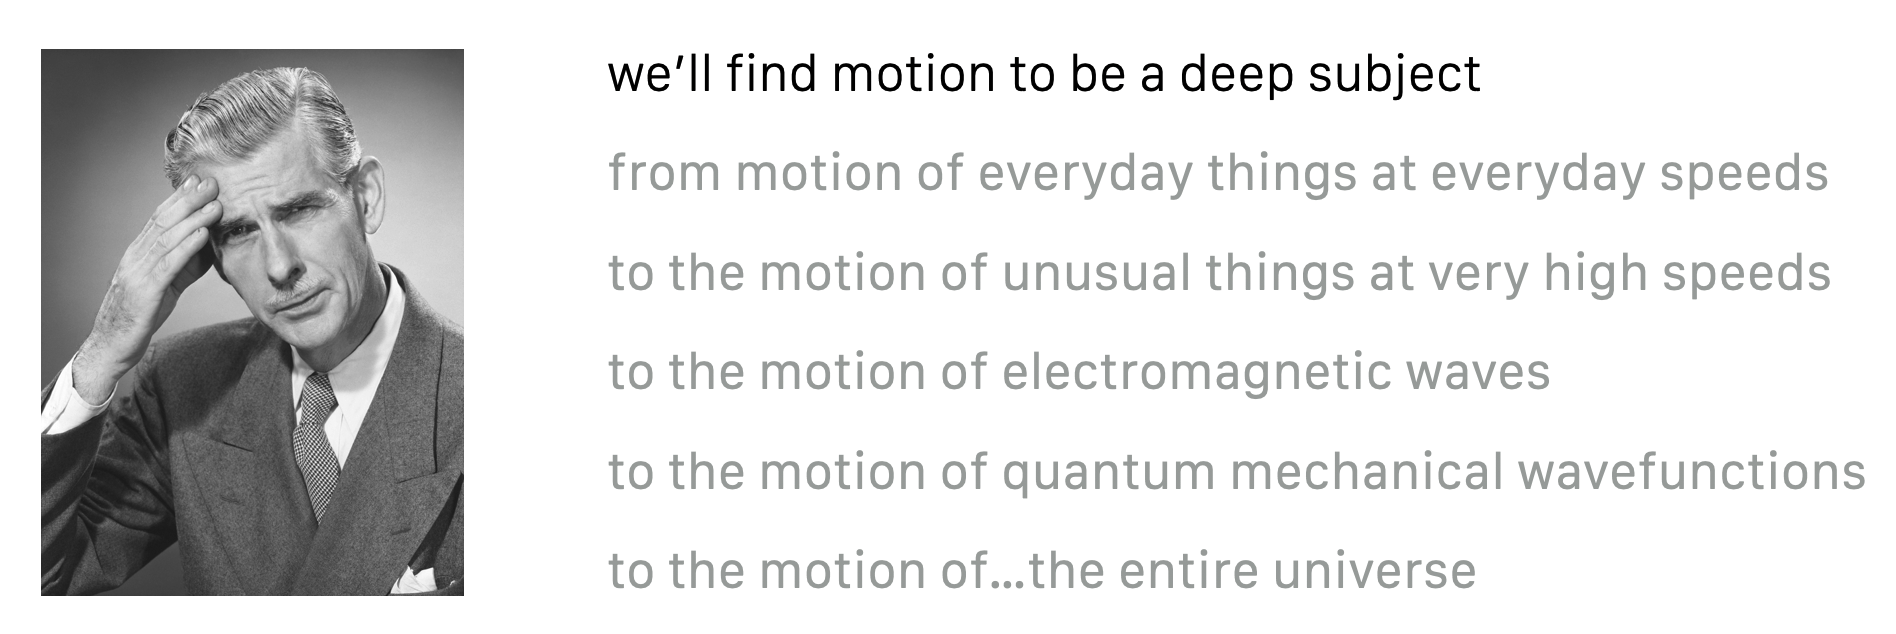
\includegraphics[width=1\linewidth,height=\textheight,keepaspectratio]{mechanics/motion/images/clipboard-2908347734.png}

Characterizing motion is simple in principle! You need two things:

\begin{figure}[H]

{\centering 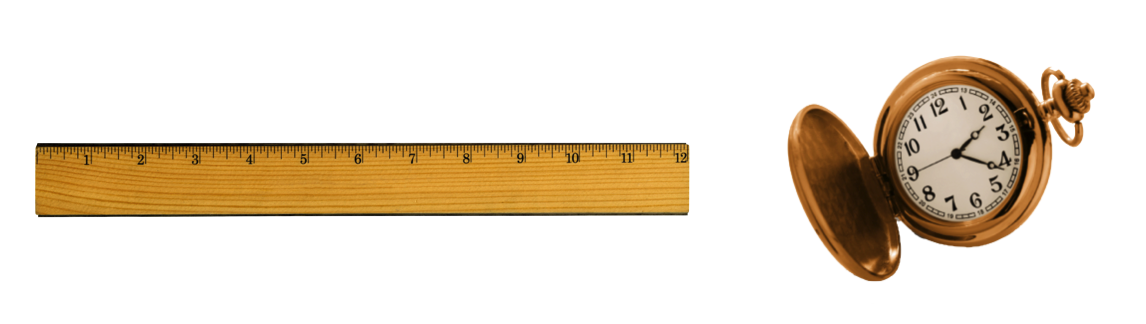
\includegraphics[width=0.8\linewidth,height=\textheight,keepaspectratio]{mechanics/motion/screenshot_3644.png}

}

\caption{All you need to measure motion.}

\end{figure}%

And for everyday motion, that seems reasonable and you already know a
lot about that.

Suppose you're on a trip and you timed yourself between the two mile
markers.

What was your speed? I know you know this and your brain would quickly
calculate:

\begin{itemize}
\tightlist
\item
  I went 350 -- 50 = 300 miies
\item
  it took me 6 hours
\item
  so my speed was 300/6 = 50 ``miles per hour,'' mph
\end{itemize}

So: \[
v=50 \text{ mph}
\] Now, what if we stop and then start up after a break? How do we refer
to the speed then?

\begin{figure}[H]

{\centering 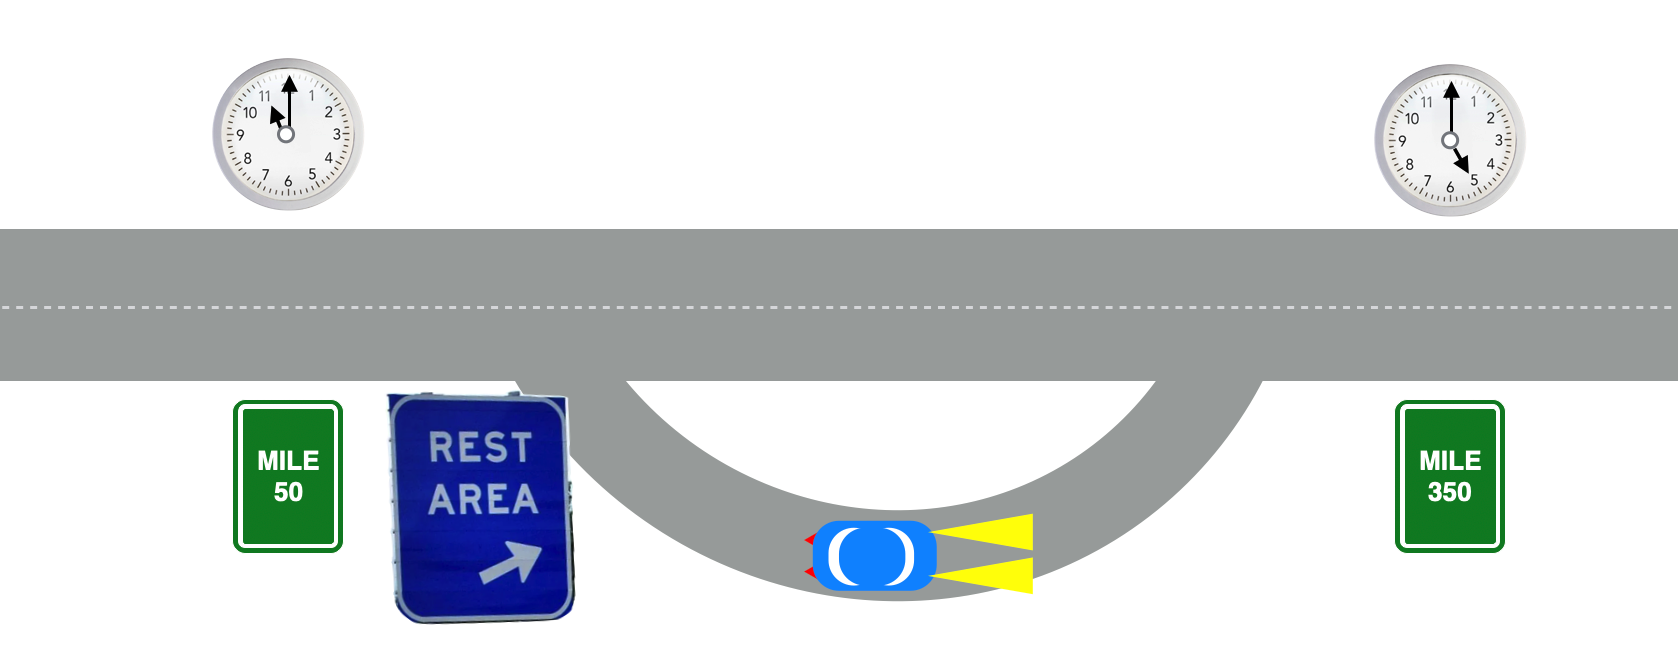
\includegraphics[width=0.8\linewidth,height=\textheight,keepaspectratio]{mechanics/motion/screenshot_3646.png}

}

\caption{Stopping for a rest}

\end{figure}%

\section{Average speed}\label{sec-averagespeed}

So as time marches on, part of it we'd be moving and part of it we'd be
stationary. But notice that the times are no different and the distances
are no different. Now your brain would be doing an average speed
calculation with exactly the same beginning and ending times and
distances. You'd now say that:

\[
<v> = 50 \text{ mph}
\]

This bracketing notation means ``average'' or ``mean''\ldots the average
speed only depends on the beginning and ending points. Since the same
number of hours elapsed, as before without the stop, we must have gone
faster than the average before the stop and/or faster after the stop.
Average speeds are not that unfamiliar, but that's because you don't
probably think of it that way. But you've all asked yourselves the
question, ``I've got to go 100 miles and I think I can travel at 70 mph,
so I''ll be home in about one and a half hours.''

So you've known for a long time that

\[
\text{speed} = \dfrac{\text{distance traveled}}{\text{time taken}}
\]

is the rate at which distance changes with time.

\subsection{Speed in Modern Terms}\label{speed-in-modern-terms}

Let's make this more compact by inserting customary symbols to get rid
of the English words. Here are some grammar rules in QS\&BB:

\begin{itemize}
\item
  We'll limit ourselves almost exclusively to motion in one dimension in
  space.
\item
  We'll use the symbol \(v\) for speed (because customarily, we'll speak
  of ``velocity''\ldots more about this below).
\item
  \(<A>\) is the average of the quantity \(A\)
\item
  We'll use the symbol \(x\) for distance in one dimension, regardless
  of which direction it points.
\item
  We'll use the symbol \(t\) for time and almost always presume that we
  set our clocks so that the beginning time of any interval is
  \(t_0=0\).
\item
  Oh, and we'll use the subscript \(\text{ }_{0}\) to indicate the
  beginning of some time or location interval---'' \(t_0\)'' or ''
  \(x_0\) ''---in a sequence of events.
\item
  We'll use the Greek symbol Delta, \(\Delta\) to mean ``change
  of''\ldots this will come up a lot.
\end{itemize}

With this, then we can ``solve'' this simple problem: \[
\begin{align}
v &= \text{speed}=\dfrac{\text{distance traveled}}{\text{time taken}} \nonumber \\
v &=\dfrac{x-x_0}{t-t_0} \label{speeddef} \\
&= \dfrac{350-50}{6}=50  \text{mph} \nonumber
\end{align}
\] where ``\(v\)'' is the velocity and it's defined by the middle
equation in equation \ref{speeddef}.

\section{Dimensional Analysis}\label{dimensional-analysis}

This might be superfluous for most of your interests, but sometimes it's
usefult to keep track of the dimensions of quantities. It can check an
answer after a calculation --~if the dimension of a result shoudl be mph
but it comes out to be ``feet'' then you made a mistake somewhere. But
it's also useful to keep track of changing from one set of units to
another, like miles per hour to meters per second.

The usual way of keeping track of the dimensions is a different kind of
bracket: \([A]\) would refer to the ``dimension of \(A\)''.

So if our distance units were feet and our time units were hours, then
we would say that the dimensions of velocity could be determined to be:
\[
\dfrac{[\text{distance}]}{[\text{time}]}=\dfrac{\text{feet}}{\text{hours}} = [v] = \text{feet per hour}
\]

\section{Spacespace and Spacetime Diagrams}\label{sec-spacetimediagrams}

There are multiple ways to represent motion\ldots{} an equation like
Equation \ref{speeddef} is a model. But graphical representation is also
very useful. Here are two:

\subsection{spacespace diagram,
stationary}\label{spacespace-diagram-stationary}

Let's imagine a pool table. Here it is with a set of x-y axes. Notice
that I've placed a ball at the intial coordinates
(\emph{x}\textsubscript{0}, \emph{y}\textsubscript{0}):

Wait a while\ldots here it still is:

\begin{figure}[H]

{\centering 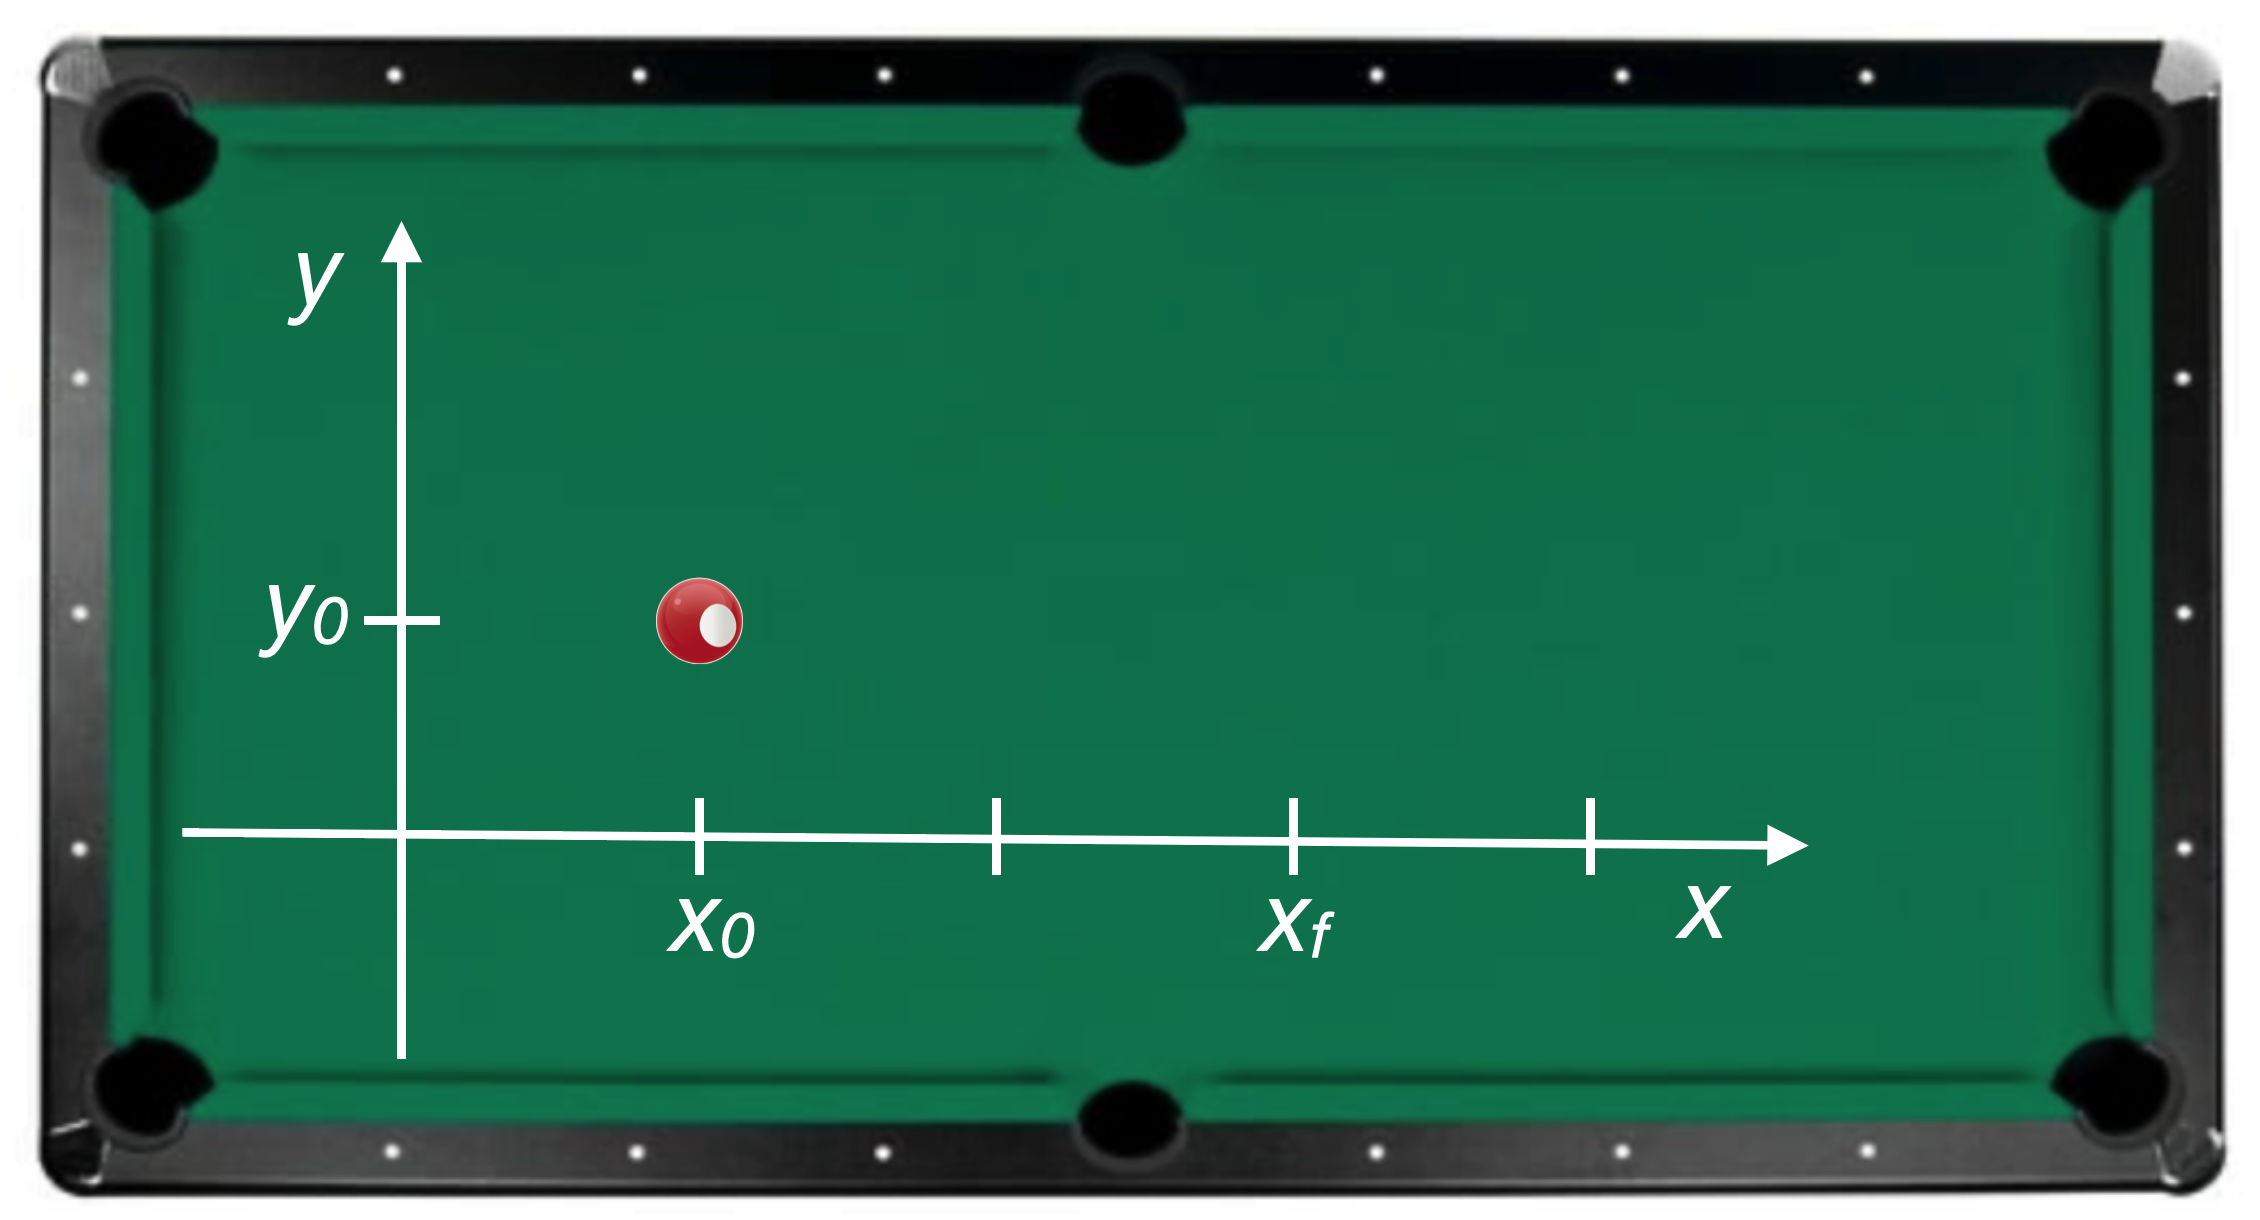
\includegraphics[width=0.8\linewidth,height=\textheight,keepaspectratio]{mechanics/motion/screenshot_3649.png}

}

\caption{Our platform for describing motion. A ball on a pool
table\ldots sitting there minding its own business.}

\end{figure}%

Let's plot it on an x-y axis set.

\begin{figure}[H]

{\centering 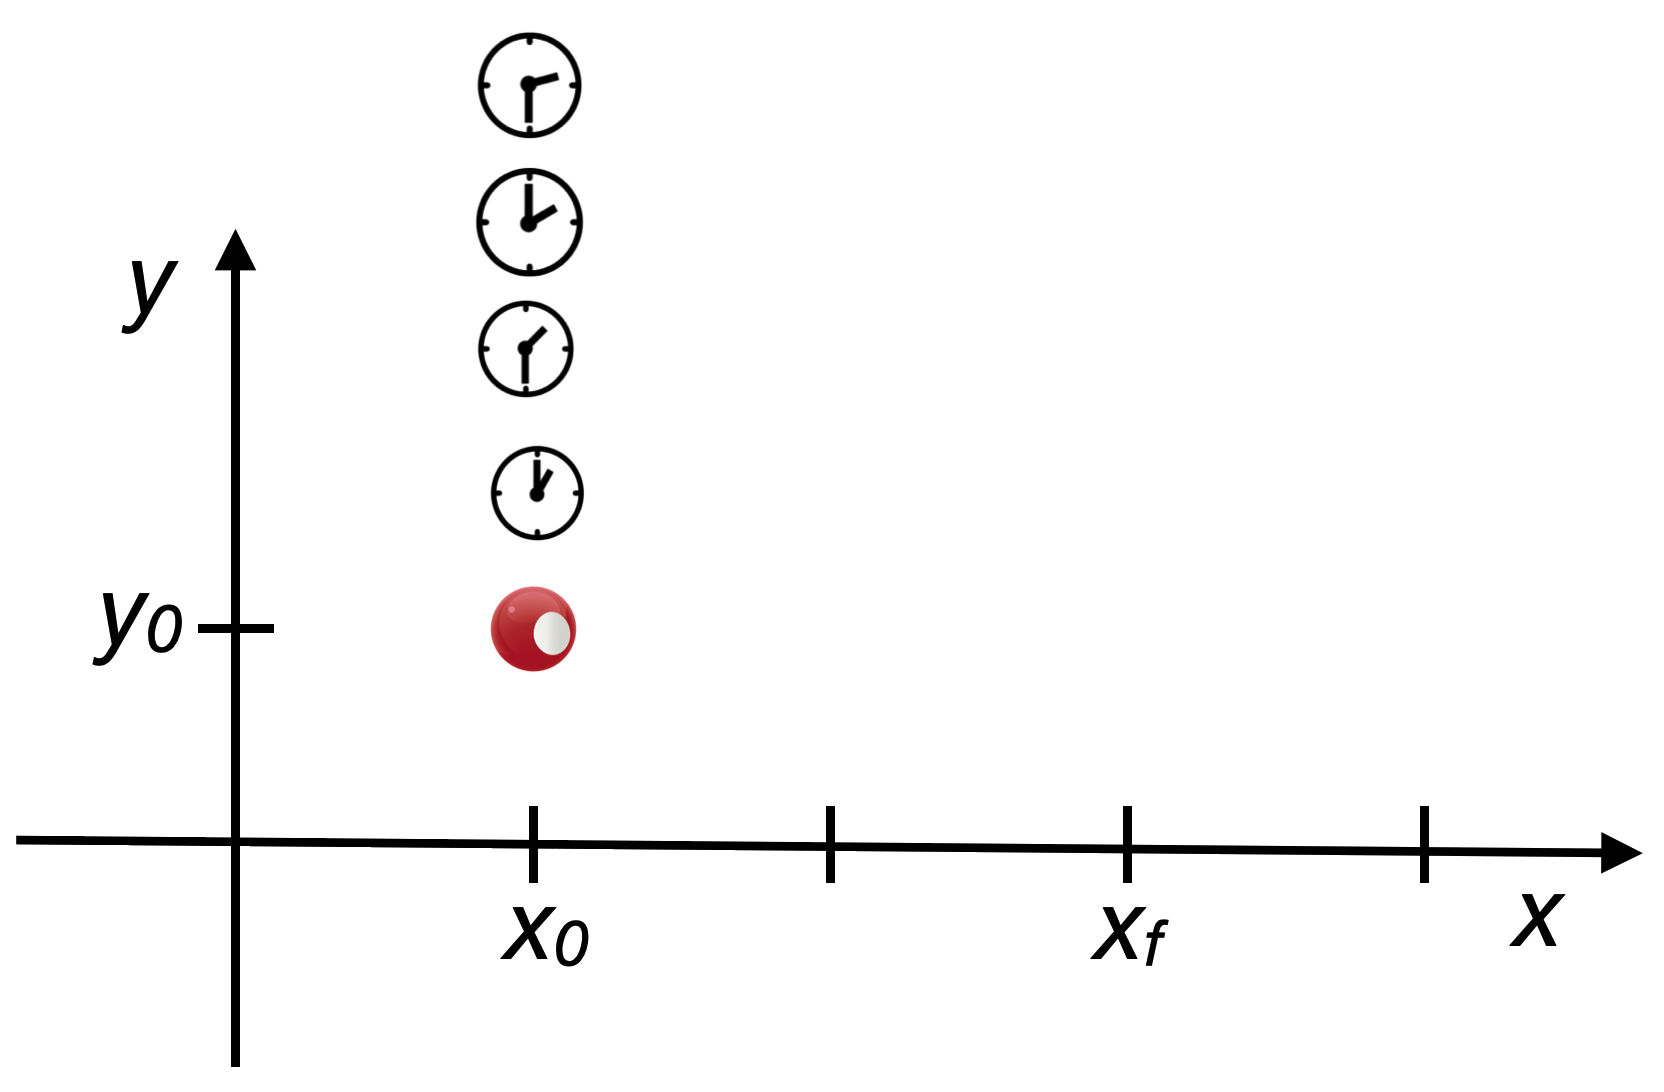
\includegraphics[width=0.8\linewidth,height=\textheight,keepaspectratio]{mechanics/motion/screenshot_3656.png}

}

\caption{A ``space-space'' diagram for the ball sitting still. Time
marches on for it in that position.}

\end{figure}%

I call this diagram a \textbf{spacespace diagram} since both axes are
space coordinates. It's how you think about things normally. As time
progresses, our ball doesn't move on the table, so the x and y
coordinates of the ball at any time are the same.

\subsection{spacetime diagram,
stationary}\label{spacetime-diagram-stationary}

Now supposed I plot the ball's trajectory (yes, ``trajectory'') as a
function of space and time.

\begin{figure}[H]

{\centering 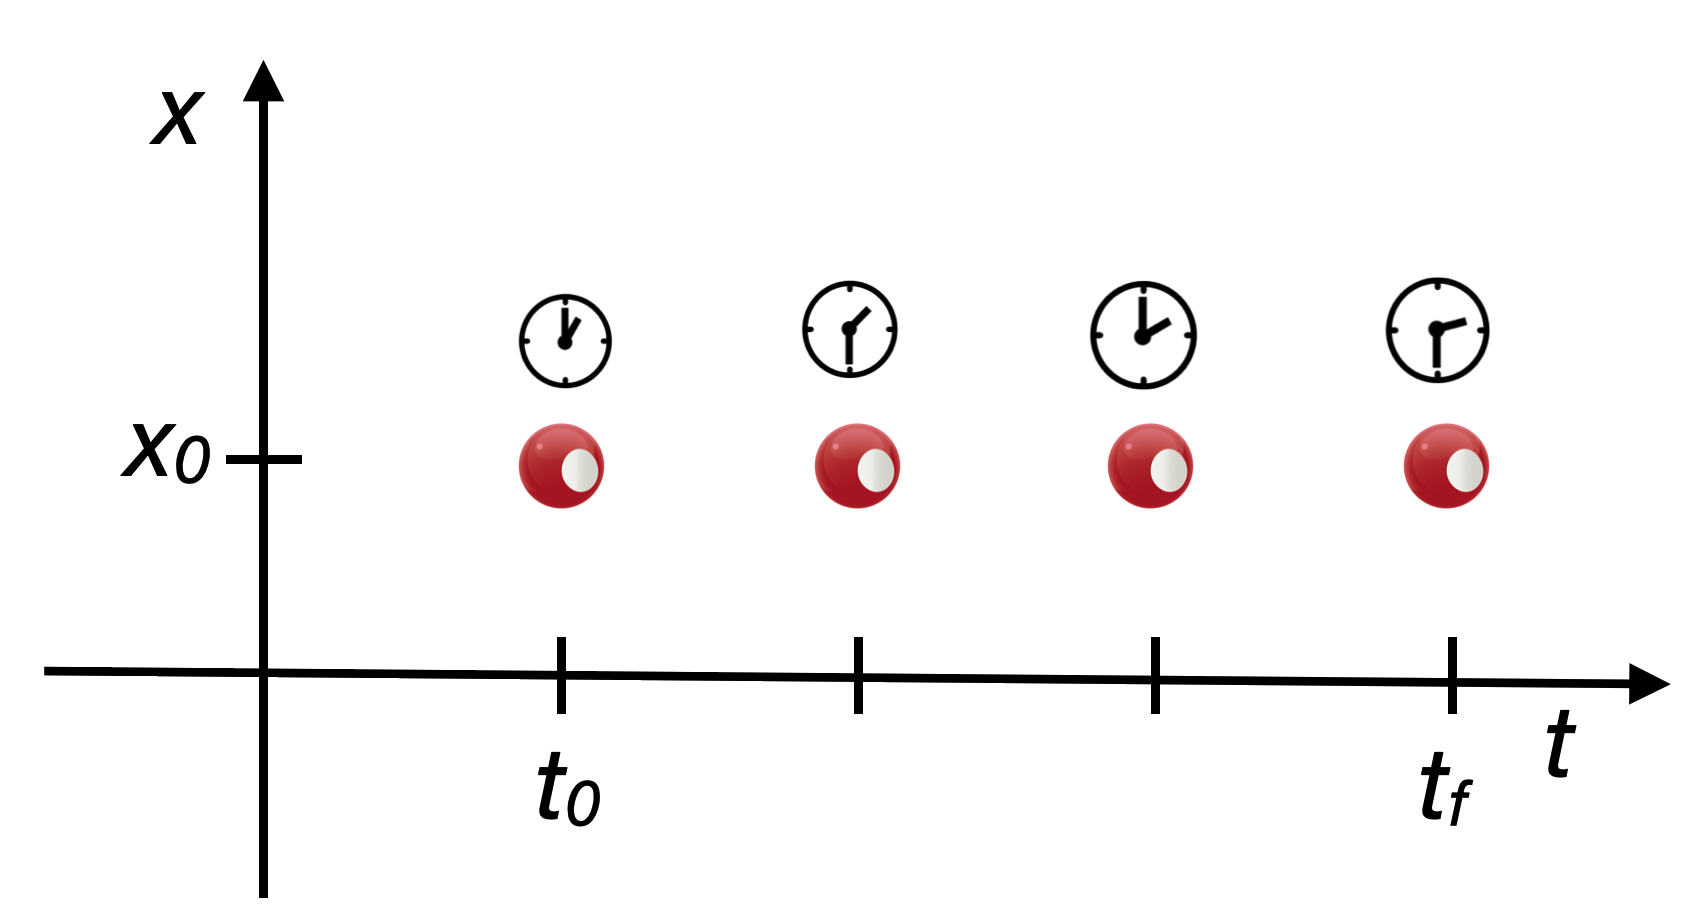
\includegraphics[width=0.8\linewidth,height=\textheight,keepaspectratio]{mechanics/motion/screenshot_3658.png}

}

\caption{A spacetime diagram for the ball sitting still\ldots still.}

\end{figure}%

Now you see ``movement''\ldots the stationary ball is moving in
\emph{time}. This picture is an example of a \textbf{spacetime diagram}.
Not very interesting.

\subsection{spacespace diagram,
moving!}\label{spacespace-diagram-moving}

Just sitting still isn't interesting, so let's roll the ball across the
pool table:

\begin{figure}[H]

{\centering 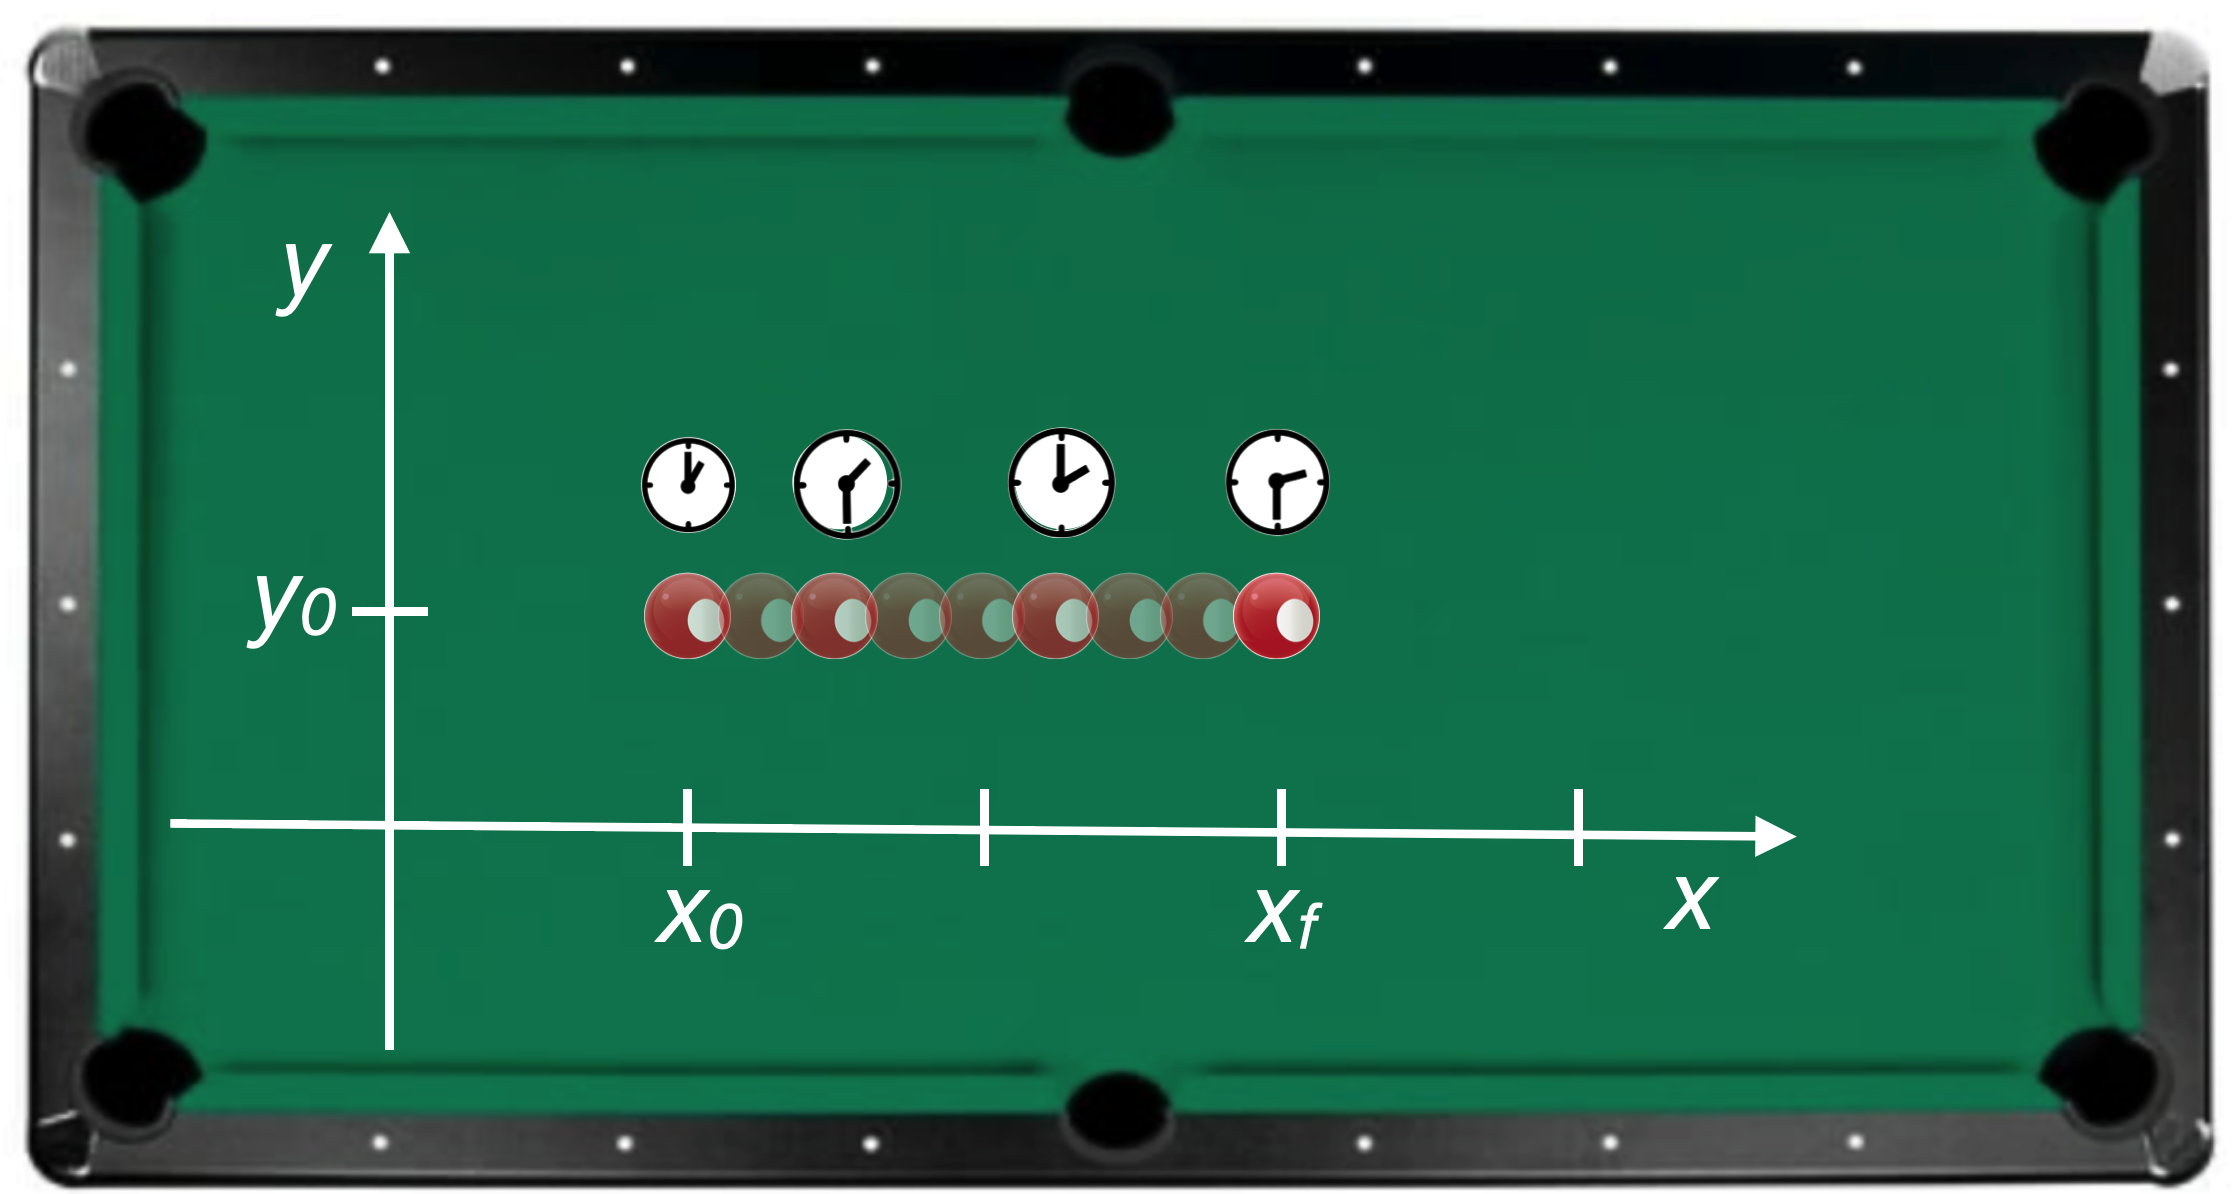
\includegraphics[width=0.8\linewidth,height=\textheight,keepaspectratio]{mechanics/motion/screenshot_3665.png}

}

\caption{Rolling the ball in a straight line on the pool table. The y
coordinate doesn't change but the x coordinate does.}

\end{figure}%

While the ball moves in space, it's also moving in time but the time
coordinate is implied or hidden. The clocks show what it might be if one
were to use a stopwatch to monitor its motion for 4 points along the
trajectory.

Since the ball moves only horizontally, \(y_0\) doesn't change and so I
can represent the motion in a space (\(x\)) and time (\(t\)) way and
here is the spacetime diagram for this simple situation

\begin{figure}[H]

{\centering 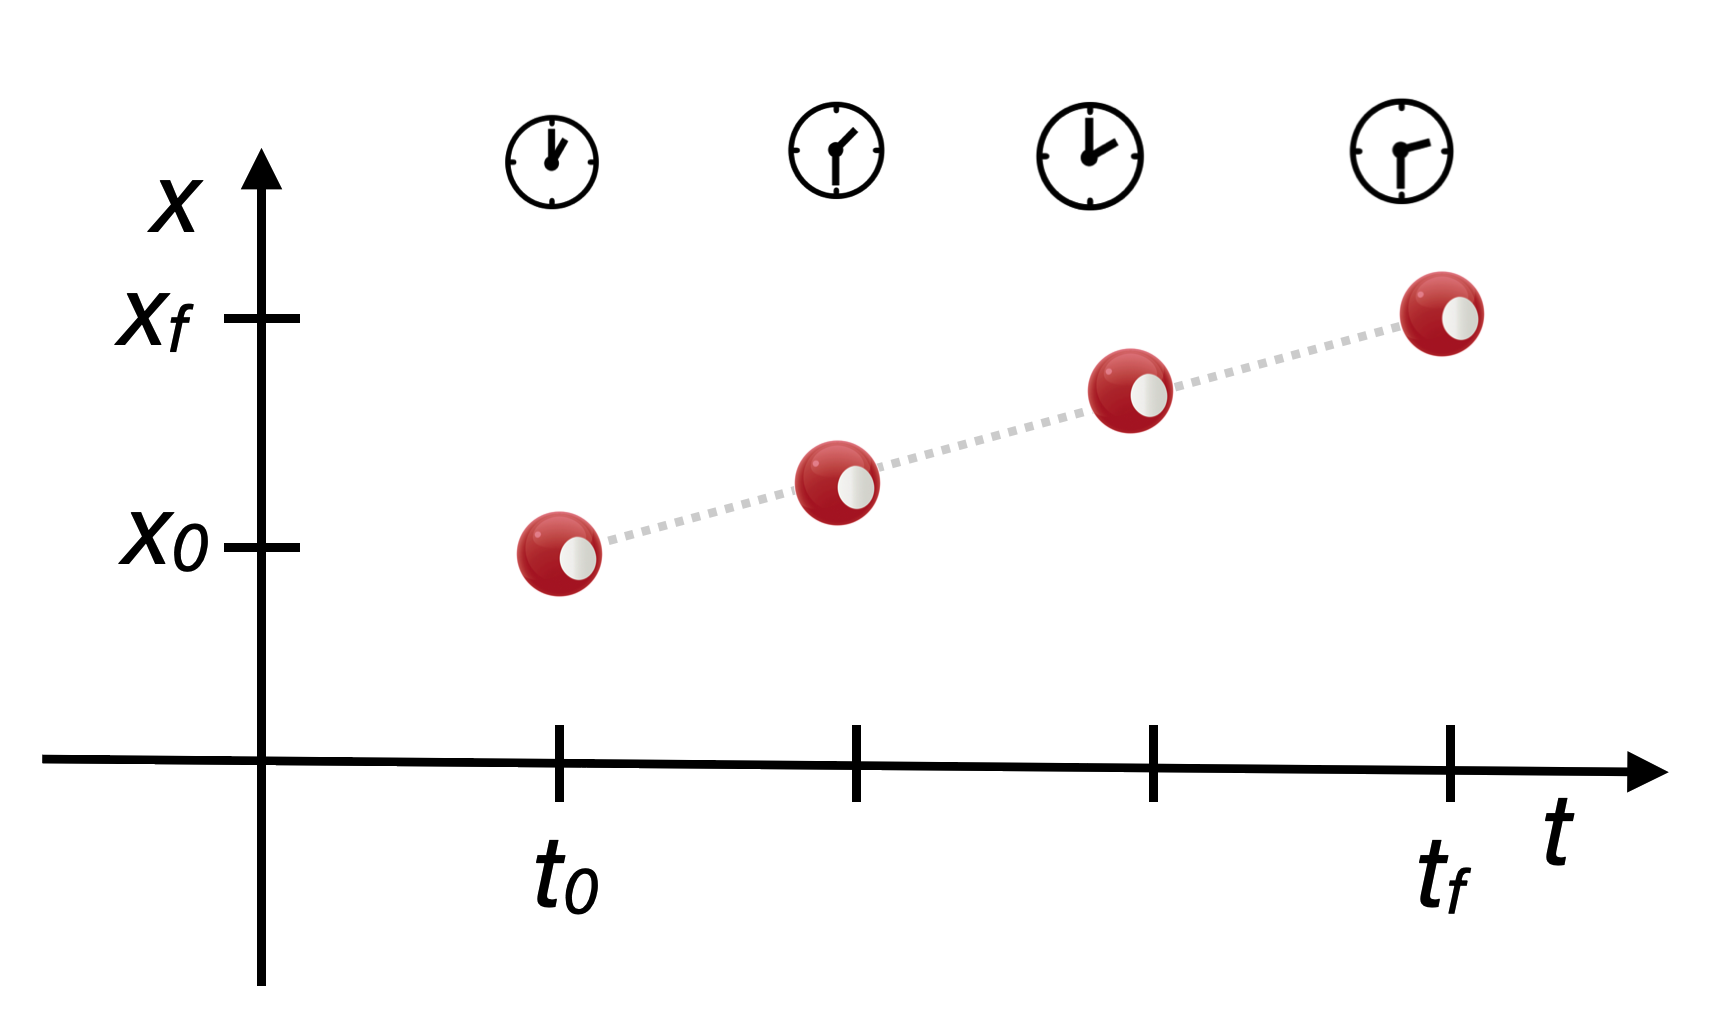
\includegraphics[width=0.8\linewidth,height=\textheight,keepaspectratio]{mechanics/motion/screenshot_3666.png}

}

\caption{The spacetime diagram for the ball moving at a constant speed
long the pool table. The x coordinate changes as time advances and the
straight line tells you that the speed is constant.}

\end{figure}%

Notice that the trajectory in spacetime is a straight line and its
slope? The velocity, which is a continuous curve in this diagram, and
the dashed line shows it.

\section{Graphing motion}\label{graphing-motion}

This is a model of motion, which for physicists is always a curve in
some coordinate system. Here the slope is \[
\begin{align}
v &=\dfrac{x-x_0}{t-t_0} \nonumber \\
v &= \dfrac{\Delta x}{\Delta t} \nonumber
\end{align}
\]

We can easily imagine that the motion might not be smooth (like the
stopping and starting on the road above) and so the concept of the
average is always in play:

\begin{figure}[H]

{\centering 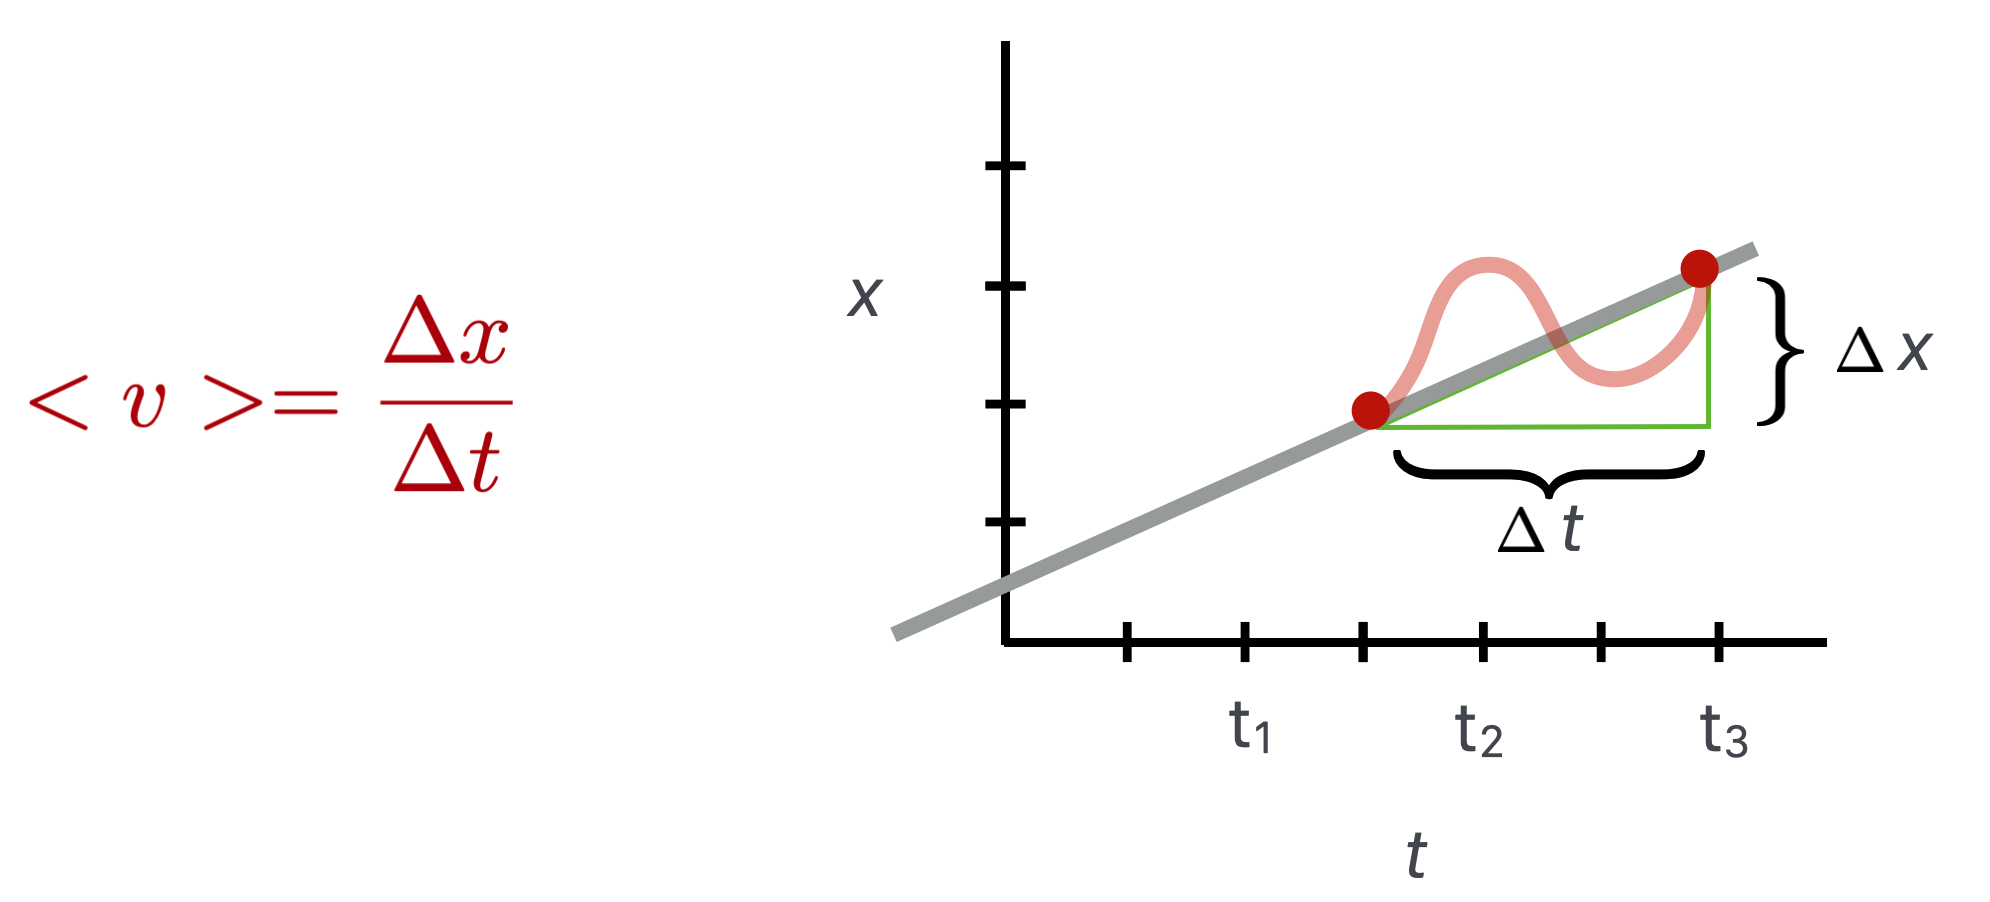
\includegraphics[width=0.8\linewidth,height=\textheight,keepaspectratio]{mechanics/motion/screenshot_3667.png}

}

\caption{The average speed depends only on the beginning and ending
points.}

\end{figure}%

The more precisely we sample the motion, the more precisely we converge
on an \textbf{instantaneous speed}, which you're familiar with while
driving with a speedometer in front of you. You think it's telling you
exaclty what your speed is, but it is actually digitally sampling the
rotation of your tires, but very finely.

In physics:

\begin{itemize}
\tightlist
\item
  ``kinematics'' is the subject of motion
\item
  ``dynamics'' is the subject of forces\ldots which cause the motion
\end{itemize}

Galileo introduced the idea of kinematics\ldots he characterized motion
without regard to what made the motion happen. Isaac Newton did the
first legitimate analysis -- model~-- of dynamics. He explained how to
characterize forces and the motions that result. That's the subject of
the next chapter.

\subsection{Acceleration}\label{acceleration}

The rolling ball's motion in spacetime had the same slope between any
two time intervals -- a straight line. So the velocity never changes.

But of course for motion to get started one has begin from rest and get
going, so the velocity has to increase in time. That's what acceleration
is.

\begin{itemize}
\tightlist
\item
  Velocity is the rate at which distance changes in time.
\item
  Acceleration is the rate at which velocity changes in time.
\end{itemize}

Here are the two models of motion: \[
\begin{align}
v &=\dfrac{x-x_0}{t-t_0} \text{  model of velocity} \label{eq1} \\
v &= \dfrac{\Delta x}{\Delta t} \text{ and } \nonumber \\
a &=\dfrac{v-v_0}{t-t_0}  \text{  model of acceleration} \nonumber \\
a &= \dfrac{\Delta v}{\Delta t} \nonumber
\end{align}
\] So if the speed is uniform, like the ball above, then the
acceleration is zero (since \(\Delta v = 0\)).

If the speed changes in time, then we have accelerated motion since
\(\Delta v \ne 0\).

Dimensions of acceleration are a little unfamiliar but we can work them
out:

\begin{figure}[H]

{\centering 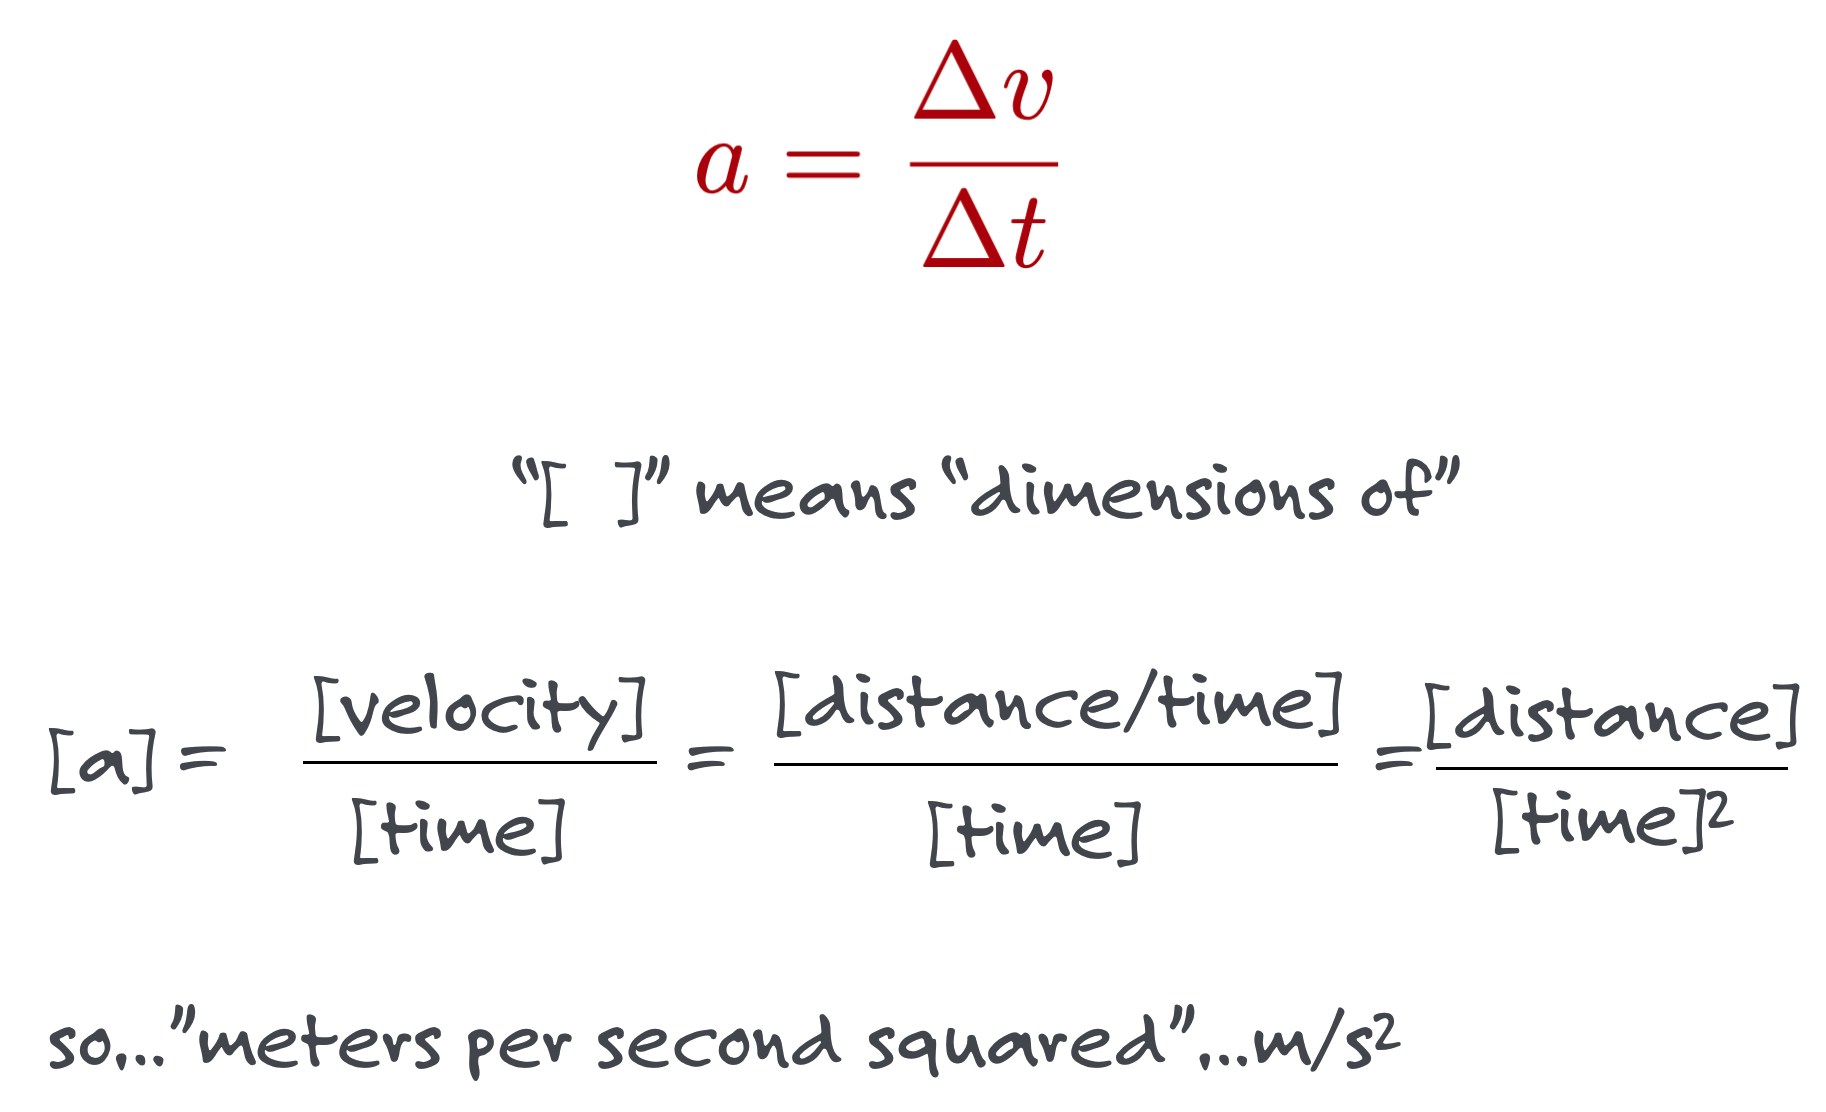
\includegraphics[width=0.8\linewidth,height=\textheight,keepaspectratio]{mechanics/motion/screenshot_3668.png}

}

\caption{screenshot\_3668}

\end{figure}%

Of course the simplest acceleration is a constant one\ldots that during
any time interval, the speed increases and the rate at which the speed
increases is constant.
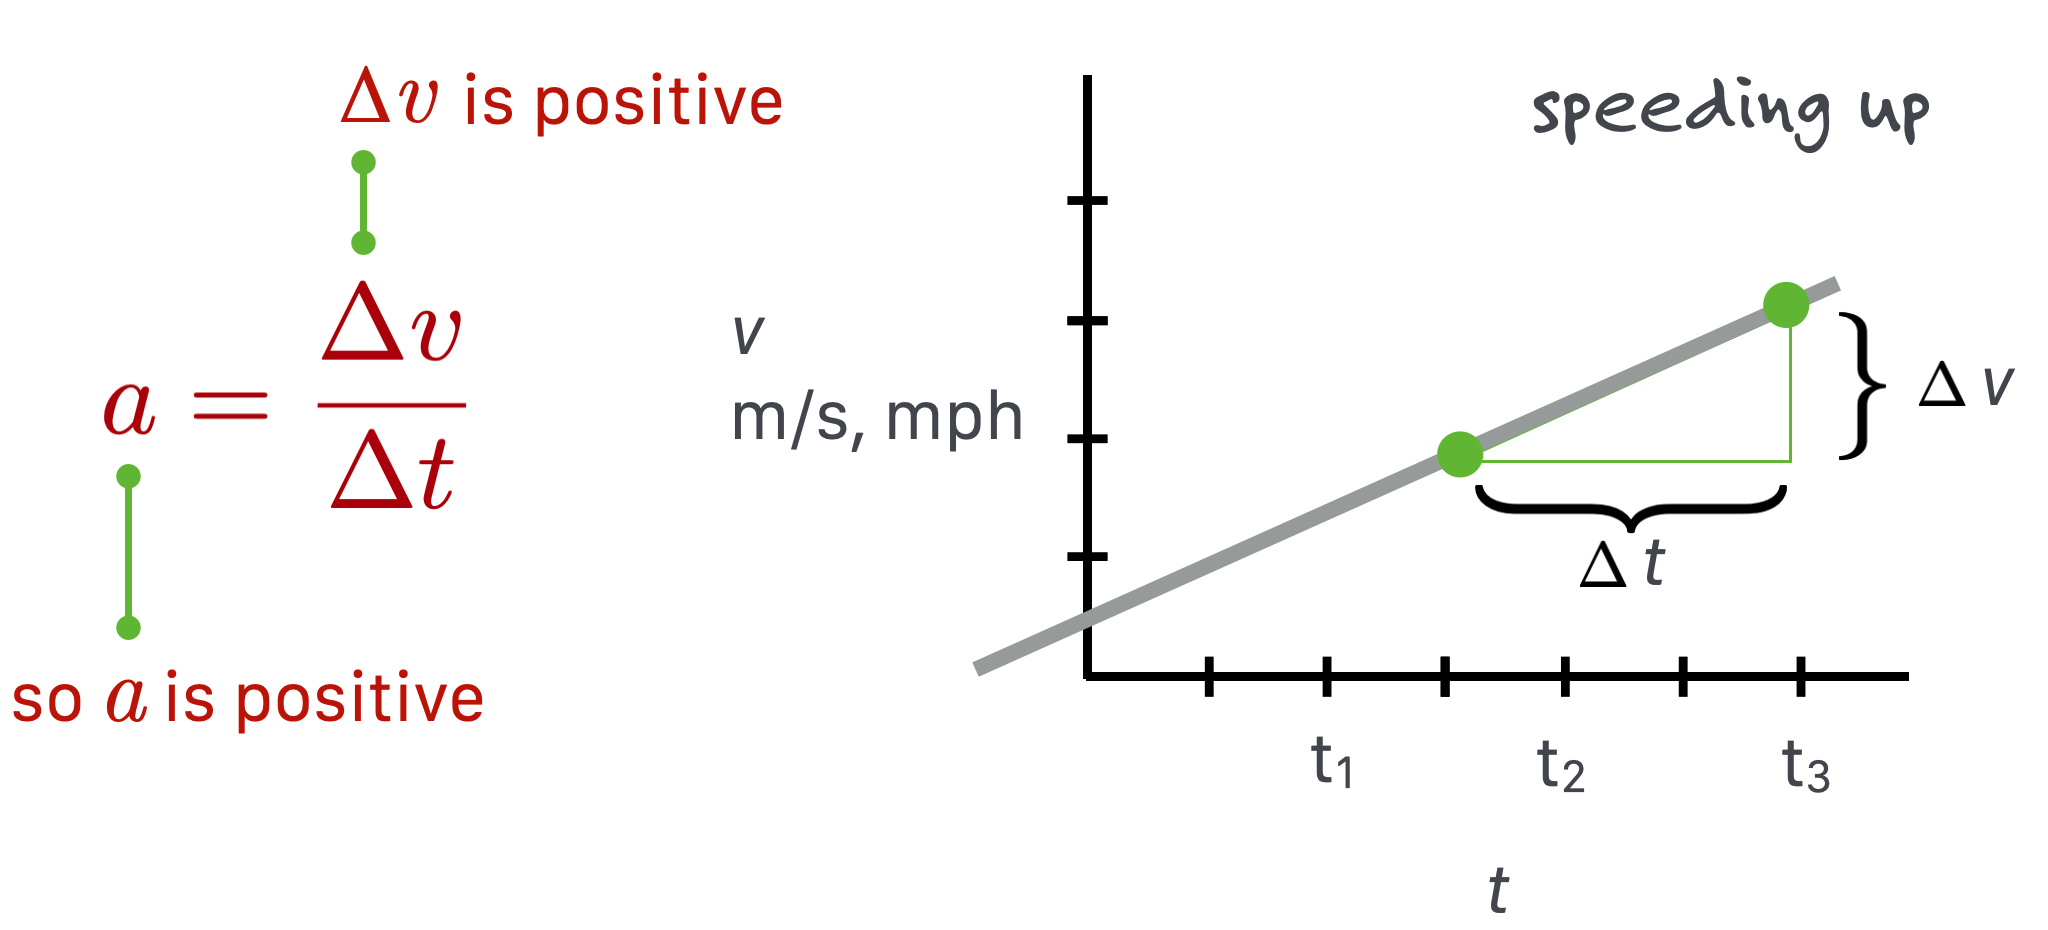
\includegraphics[width=0.8\linewidth,height=\textheight,keepaspectratio]{mechanics/motion/screenshot_3669.png}

But sometimes you put on the brakes, and you know that you slow down
because you can feel it and the speedometer is telling you that. So in
increasing time intervals, the rate at which the speed changes is
negative.

\begin{figure}[H]

{\centering 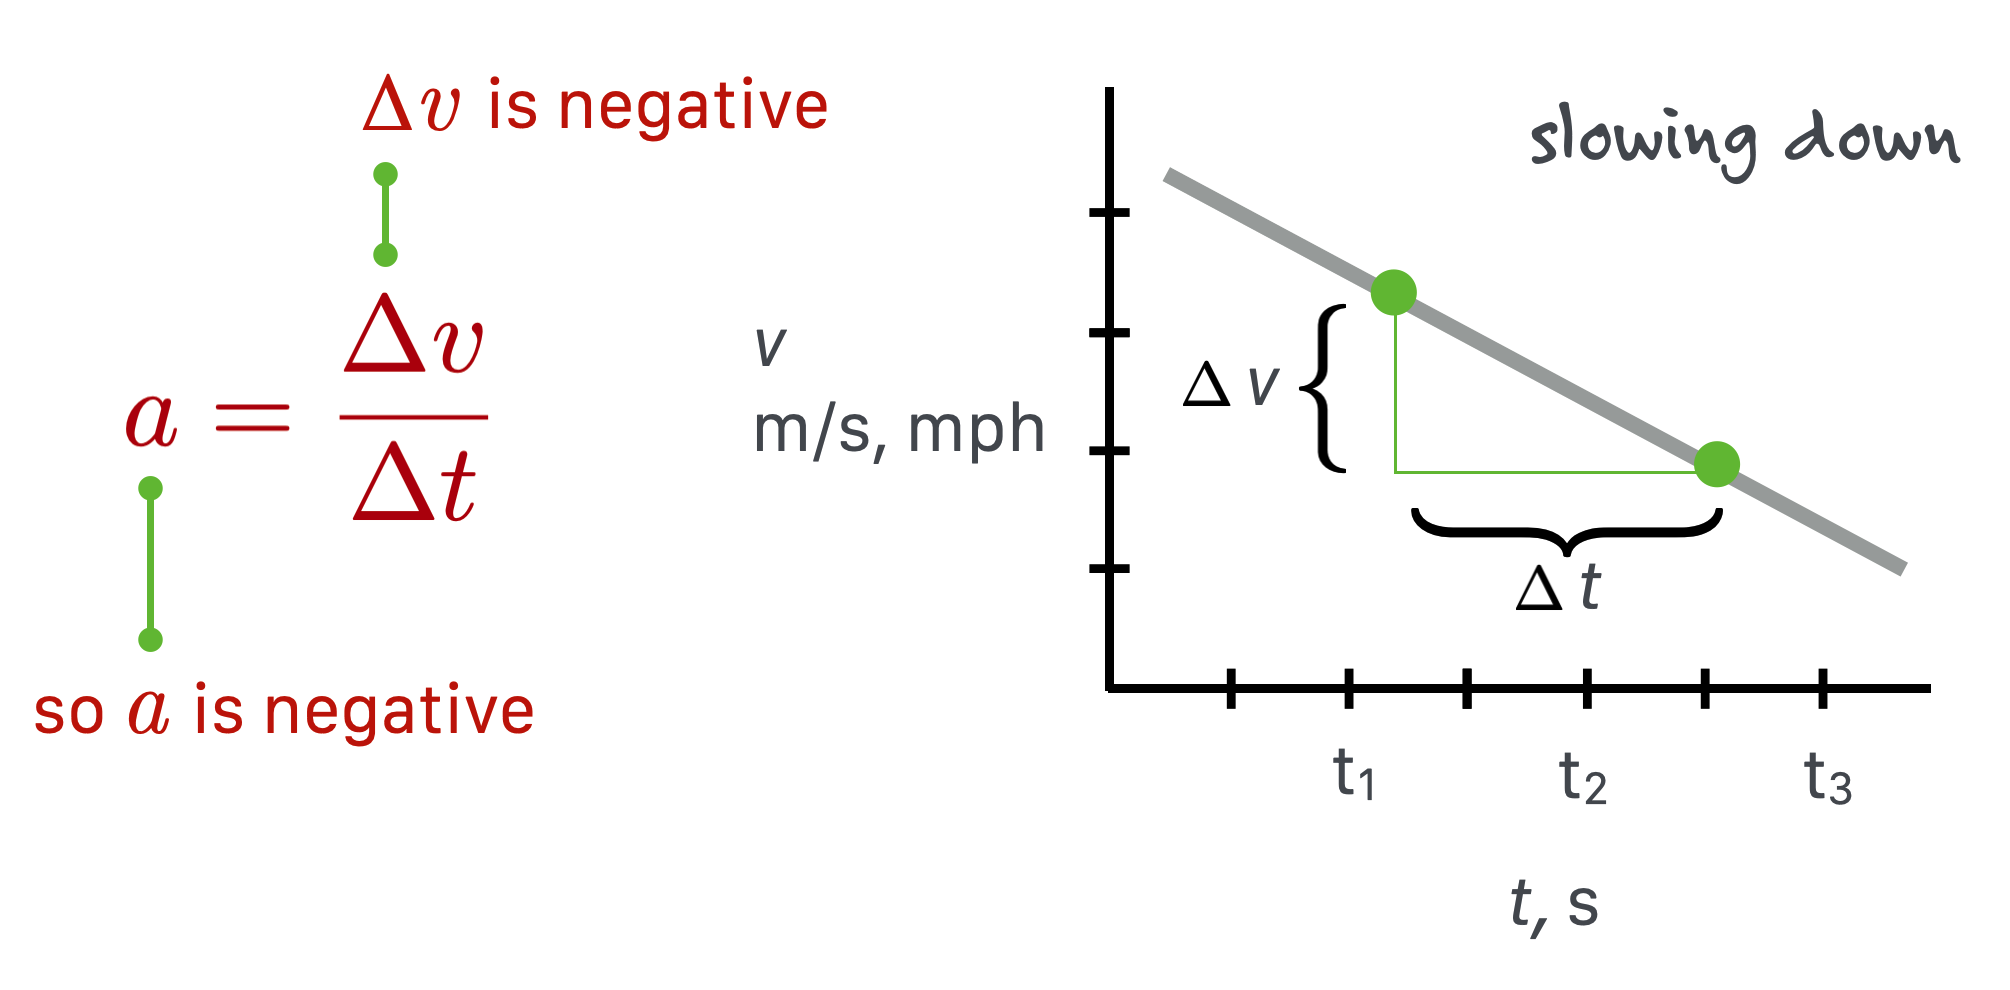
\includegraphics[width=0.8\linewidth,height=\textheight,keepaspectratio]{mechanics/motion/screenshot_3670.png}

}

\caption{screenshot\_3670}

\end{figure}%

In the diagram, \(\Delta v < 0\). This is a negative acceleration and is
called decceleration.

I've concentrated on acceleration and deceleration which are
constant\ldots the speed changes at a uniform rate, up or down. But
that's not the only kind. Think about a sprinter. Just after the
starting gun, a runner's speed out of the blocks is high and remains
high for the first few steps. As the runner starts to become a little
more vertical, air resistance becomes a factor and while the runner goes
faster, she does so at a lower rate of speed increase. That's a
non-constant acceleration.

\marginnote{\begin{footnotesize}

\begin{figure}[H]

{\centering 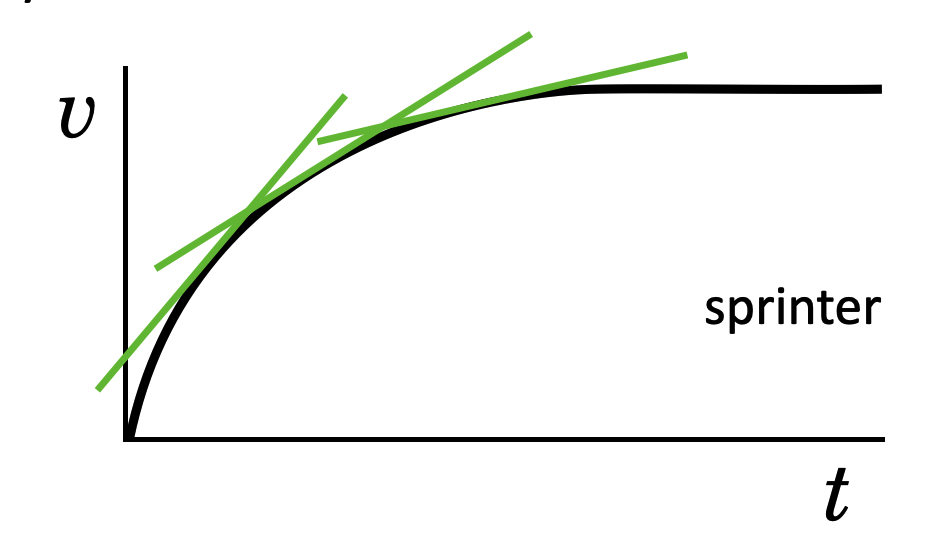
\includegraphics[width=0.8\linewidth,height=\textheight,keepaspectratio]{mechanics/motion/screenshot_3671.png}

}

\caption{A sprinter's changing acceleration. Notice that the slope
changes as time inncreases}

\end{figure}%

\end{footnotesize}}

Now you can design a sports video game. All you have to do is measure an
athlete's personal acceleration parameters and code them. I found this
years ago for Madden NFL11 of a particular running
back: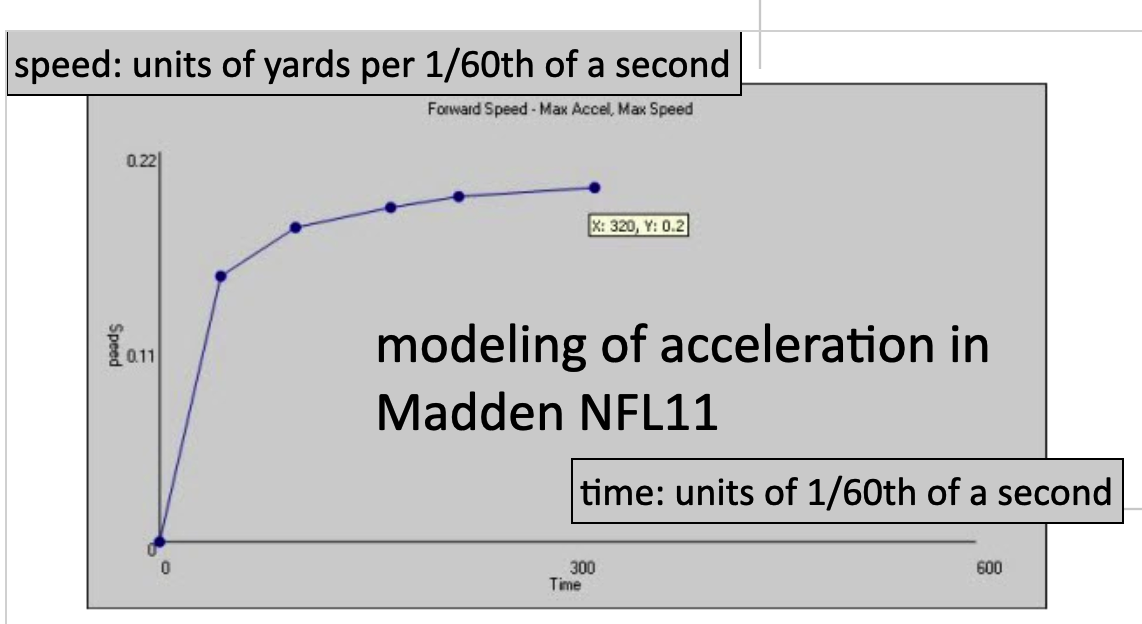
\includegraphics[width=0.8\linewidth,height=\textheight,keepaspectratio]{mechanics/motion/screenshot_3672.png}

\section{Gravity}\label{gravity}

Famously, Galileo Galilei determined that any object near the earth
would fall at a constant acceleration. How he determined this was clever
and you can read the story at
\href{../../history/galileo_free_fall.qmd}{Galileo}. What he found was
that the speed of a falling object would increase linearly with the time
of it's fall. A competing idea from other natural philosophers including
Leonardo DaVinci, proposed that the speed would increase linearly
\emph{with distance, not time}.

What Galileo knew from medieval considerations was that this linearity
with time for \(v\) meant that distance had to increase quadratically
with time.

So, a model of Galileo's qualitative conclusion is: \[
\begin{align}
v(t) &\propto t \nonumber \\
x(t) &\propto t^2 \nonumber
\end{align}
\] The symbol \(\propto\) means ``proportional to'' and when we find a
relationship like that, we can turn it into an equation by inserting
some constant of proportionality. For falling bodies near the earth, the
symbol for that constant is called ``\(g\)'' or ``little g.'' Now we can
fully-form the model as: \[
\begin{align}
v(t) &= gt \nonumber \\
x(t) &= 1/2gt^2 \nonumber
\end{align}
\] There are simplicity reasons for the 1/2\ldots if we'd absorbed that
into \(g\) then the first equation would have had to change. The value
of \(g\) comes from experiment and is about \[
\begin{equation}
g = 9.8 \text{ m/s$^2$} = 32 \text{ ft/s$^2$}.  \nonumber \\
\end{equation}
\] While this is a story that started with gravity, it's nonetheless a
completely general description of any accelerated motion (your car) if
that acceleration is constant. In general, then, we'd use the symbol
\(a\) and treat falling as a special case of constantly accelerated
motion in which case \(a=g\).

While we defined speed in terms of distance, we can rewrite Equation
\ref{eq1}. \[
\begin{align}
\text{For constant speed,}&\text{ no acceleration} \\
v &=\dfrac{x-x_0}{t-t_0} \nonumber \\
x-x_0 &=v(t-t_0) \nonumber \text{ let's take our initial time be 0} \\
x &= x_0 + vt
\end{align}
\] And for constant acceleration, we can find a general relationship for
distance as well with a simple calculation.

\begin{tcolorbox}[enhanced jigsaw, toprule=.15mm, opacityback=0, colframe=quarto-callout-warning-color-frame, rightrule=.15mm, coltitle=black, bottomtitle=1mm, colbacktitle=quarto-callout-warning-color!10!white, bottomrule=.15mm, toptitle=1mm, titlerule=0mm, title={Warning}, arc=.35mm, leftrule=.75mm, left=2mm, colback=white, breakable, opacitybacktitle=0.6]

⚠️ A bit of algebra is required to derive the complete quartet of
equations for motion with a constant acceleration. I do that for you in
\href{./Motion_equations.qmd}{equations of motion}

\end{tcolorbox}

\section{Complete model for motion}\label{sec-equationsofmotion}

So collectively, here are our definitions for motion: \[
\begin{align}
\text{Constant speed,}&\text{ no acceleration} \nonumber \\
x &= x_0 + vt \nonumber \\
v &= \text{ constant} \nonumber \\
a &= 0 \nonumber \\
\text{Constant}&\text{ acceleration}& \nonumber \\
a &=\dfrac{v-v_0}{t-t_0} \nonumber \\
a &= \dfrac{\Delta v}{\Delta t} \nonumber \\
\end{align}
\] And here are the complete set of equations for one-dimentional
constant acceleration. Each relation relates two of the three variables:
\(x, t, v\). \[
\begin{align}
& \text{1. } \; x = \langle v \rangle t \label{avev} \\ 
& \text{2.  } \; v   = v_0 + at \label{vat} \\
& \text{3. }  \; x   = x_0+v_0 t + \frac{1}{2} at^2 \label{xat}  \\
& \text{4. }\; v^2   = v_0^2 + 2ax \label{vax} 
\end{align}
\]

Notice two things. If the motion is at a constant velocity, then setting
\(a=0\) recovers that special case. And notice that \eqref{vax} does not
have time as a variable and that will turn out to be interesting when we
talk about energy.

\begin{center}\rule{0.5\linewidth}{0.5pt}\end{center}

\section{Projectiles}\label{sec-projectiles}

When you throw a ball from centerfield to home plate, the ball executes
what looks like a parabollic trajectory. The ball goes forward while it
probably rises for a while and then drops toward the ground. That's
two-dimensional motion and Galileo had the insipiration to figure out
what was going on and how to do experiments to confirm his hypothesis
that the up-and-down would follow the shape of a parabola.

His insight was that when motion is imparted to an object and the source
of the motion is taken away (you throw the ball and it leaves your hand
and is then in its own), that something stays with the ball. He called
it ``impeto'' and we call it ``momentum.'' The ball acquires momentum.

And he realized that whatever impeto the ball acquires in the horizontal
direction is preserved, but the moment the ball leaves your hand, it
starts to head toward the Earth. In modern words, we'd say that once
released, the ball has a horizontal momentum that stays constant and a
vertical momentum that changes and points down. The two motions are in
some sense overlaid or shared by the ball.

{
\makeatletter
\def\LT@makecaption#1#2#3{%
  \noalign{\smash{\hbox{\kern\textwidth\rlap{\kern\marginparsep
  \parbox[t]{\marginparwidth}{%
    \footnotesize{%
      \vspace{(1.1\baselineskip)}
    #1{#2: }\ignorespaces #3}}}}}}%
    }
\makeatother

\begin{figure}

\sidecaption{\label{fig-motion_head2}Throwing a ball. The vertical axis
is the height above the ground and the horizontal axis is the range. The
curve shows the trajectory of a thrown ball in the absence of any air
resistance -- a perfect parabola. The intitial velocity is shown as the
arrow at location 1. At each of the five points the overall velocity is
broken into horizontal and vertical components.}

\centering{

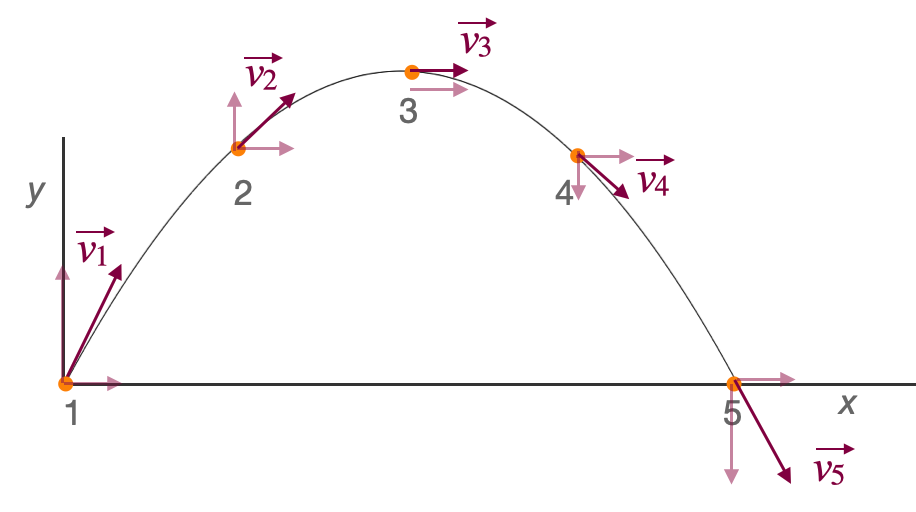
\includegraphics[width=1\linewidth,height=\textheight,keepaspectratio]{mechanics/motion/screenshot_3677.png}

}

\end{figure}%

}

In the figure you can see that the original velocity \(v_1\) points up
and foward and I've broken up this arrow (a vector) into it's horizontal
component which you can see at 1, 2, 3, 4, and 5 is the same length.
It's ``impeto'' is constant. The vertical component changes at each
point -- disappearing at the top --~and then increasing down as the ball
heads to Earth. Gravity wins.

For QS\&BB we'll not need two dimensional kinematics.

\chapter{The Big Mo: Momentum and
Force}\label{the-big-mo-momentum-and-force}

Author: Chip Brock · Drafted: April 15, 2025

\begin{center}\rule{0.5\linewidth}{0.5pt}\end{center}

\marginnote{\begin{footnotesize}

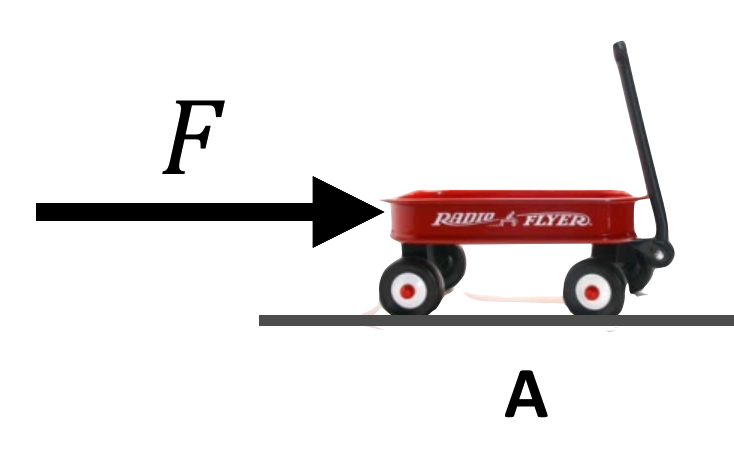
\includegraphics[width=1\linewidth,height=\textheight,keepaspectratio]{mechanics/momentum/screenshot_3679.png}

\end{footnotesize}}

This is the first of three outlines of some basic physics ideas so that
I can refer to them in other posts. If you'd like more, including
history and examples, then visit
\href{https://qstbb.pa.msu.edu/storage/ISP220_fall2020/QS&BB2020/intro.html}{full
textbook} for a textbook-level presentation. If you only need the basic
simple equations, they're here. If you'd like some explanation, that's
next!

\chapter{Skinny Momentum and Force}\label{skinny-momentum-and-force}

Units. Sorry. In QS\&BB we won't care about English versus metric units
but for this motion review we'll sometimes have to convert. I'll do it
for you but you can check me at places like
\href{https://www.unitjuggler.com/index.html}{unitjuggler}\ldots or
often just Google.

\section{Just the facts:}\label{just-the-facts-1}

\subsection{some defintions}\label{some-defintions}

\begin{itemize}
\tightlist
\item
  mass, \(m\), is the quantity of matter\ldots but this concept changes
  over history and is somewhat circular. It has a couple of jobs to do.
\item
  Job 1: inertia is the reluctance of an object to move and the measure
  of interia is mass.
\item
  Job 2: impulse is related and sort of intuitive: push on something
  hard and it will go faster, push on something for a long time and it
  will go faster: \(F\Delta t\) is proportional to the change in
  velocity and the proportionality constant is \(m\)
\end{itemize}

\subsection{impulse}\label{impulse}

\[
\begin{equation}
F\Delta t = m\Delta v
\end{equation}
\]

\subsection{momentum}\label{momentum}

\$\$ \begin{align}
F\Delta t &= \Delta (mv) \nonumber \\
p &= mv \\
F\Delta t &= \Delta p \\

\end{align} \$\$

\subsection{force}\label{force}

from the above: \[
\begin{align}
\text{rearranging impulse: }F &= \frac{\Delta p}{\Delta t} \\
\text{if the mass is constant } F &= ma
\end{align}
\]

\section{Pointers to topics:}\label{pointers-to-topics-1}

\begin{tcolorbox}[enhanced jigsaw, toprule=.15mm, opacityback=0, colframe=quarto-callout-tip-color-frame, rightrule=.15mm, coltitle=black, bottomtitle=1mm, colbacktitle=quarto-callout-tip-color!10!white, bottomrule=.15mm, toptitle=1mm, titlerule=0mm, title={Tip}, arc=.35mm, leftrule=.75mm, left=2mm, colback=white, breakable, opacitybacktitle=0.6]

🔐 Bottom line sections with stuff to remember in this chapter:

\begin{itemize}
\item
  average speed Section~\ref{sec-averagespeed}
\item
  spacespace and spacetime diagrams Section~\ref{sec-spacetimediagrams}
\item
  the set of equations for 1-dimensional motion
  Section~\ref{sec-equationsofmotion}
\item
  2 dimensional motion: projectiles Section~\ref{sec-projectiles}
\end{itemize}

\end{tcolorbox}

\chapter{Gentle explanations of Momentum and
Force}\label{gentle-explanations-of-momentum-and-force}

\section{Isaac Newton's important
idea}\label{isaac-newtons-important-idea}

To start something moving from rest? Apply a force. To speed up or slow
down something already moving? Apply a force! To cause something to
deviate from a straight line? Yes. Another force. To keep something
moving at a constant speed? No (net) force required, thank you.

Here's what he said:

\begin{tcolorbox}[enhanced jigsaw, toprule=.15mm, opacityback=0, colframe=quarto-callout-important-color-frame, rightrule=.15mm, coltitle=black, bottomtitle=1mm, colbacktitle=quarto-callout-important-color!10!white, bottomrule=.15mm, toptitle=1mm, titlerule=0mm, title={Important}, arc=.35mm, leftrule=.75mm, left=2mm, colback=white, breakable, opacitybacktitle=0.6]

🫵 Whenever there's a change of velocity on any object, a force is at
work: since acceleration is a change in velocity, forces are responsible
for acceleration. Note: because velocity is technically a vector, then
changing direction is also changing velocity.

\end{tcolorbox}

One of the many ways that Newton got into the textbooks was to argue
with Aristotle who insisted that \emph{all motion} requires a pusher in
physical contact: No, Newton said. Constant motion \emph{is} free. It's
only accelerated motion that requires payment in the form of the action
of a force.

Let's start slowly and sneak up on this idea. Impulsively.

\subsection{Impulse -- Every sport}\label{impulse-every-sport}

In QS\&BB we don't need much depth, but we do need three important
concepts\ldots the ones that underpinned Newton's system:
\textbf{force}, \textbf{mass}, and \textbf{momentum}. Let's move:

In the previous lesson we laid out the rules that govern an object's
motion.

Newton: To get something up to speed, you need to whack it or shove it
--- either \emph{a sharp collision or a steady push} increases the speed
of an object. Push harder? More speed. Push longer? Again, more speed.

So let's codify that everyday notion into a model of forces and motion.
Let's imagine a force, \(F\) that pushes during some time interval,
\(\Delta t\). A whack means that \(\Delta t\) is small (like a golf club
hitting a ball) while a steady shove (like a rugby scrum) means that the
force is slowly applied so \(\Delta t\) is larger.

Here's what we know from experience: applying a force (\(F\)) to
something for a time interval (\(\Delta t\)) results in the speed
increasing in proportion, (\(\Delta v\)). We have the beginnings of a
model:

\[
\begin{equation}
F\Delta t \propto \Delta v. \label{eq:impulse1}
\end{equation}
\]

Increase \(F\), \(\Delta t\), or both on the left-hand side, and the
speed goes up on the right-hand side. The quantity on the left side is
called the \textbf{Impulse}. It's the sports-quantity. Any game
involving a ball involves impulse and exceptional athletes can control
both the \(F\) and the \(\Delta t\). The quantity on the right implies
that the speed changed and of course if the speed changed, then the
object accelerated and/or it changed direction.

We need to refine the model. But first some units and language:

\begin{quote}
\textbf{May the force be with you by so many different names} We will
use forces many times in QS\&BB, which is a common quantity in our lives
because of ``weight.'' But if you're from the United States, when you
step on the bathroom scale it reports back to you your weight in the
Imperial measurement system (or ``customary measures system'') as too
many \textbf{Pounds}, lbs. In a minute, you'll see why that's confusing
when comparing to the rest of the world where the bathroom scale would
report kilograms. The unit of force in the International System of Units
(SI), which includes the older ``metric system'' or MKS (Meter,
Kilogram, Second) is the \textbf{Newton}, N. If you go to the gas
station in Berlin, you'll fill your tires to a pressure measured in
Pascals, which is Newtons per square meter. Of course up the street from
me, our Michigan gas station reports pounds per square inch for my
pressure.
\end{quote}

We'll predominantly use the unit of Newton as the modern measure of a
force -- like the rest of the civilized world. I'll not obsess with
units and so I'm happy for you to rely on Mr.~Google in almost all
instances.

\begin{tcolorbox}[enhanced jigsaw, toprule=.15mm, opacityback=0, colframe=quarto-callout-important-color-frame, rightrule=.15mm, coltitle=black, bottomtitle=1mm, colbacktitle=quarto-callout-important-color!10!white, bottomrule=.15mm, toptitle=1mm, titlerule=0mm, title={Important}, arc=.35mm, leftrule=.75mm, left=2mm, colback=white, breakable, opacitybacktitle=0.6]

🔐 Type this into your browser: ``convert 10 pounds into newtons'' and
you'll be rewarded with the answer and a tool for all kinds of unit
conversions. You're welcome.

\end{tcolorbox}

\subsection{Inertia}\label{inertia}

\emph{Pressing} forward (see what I did there?). Let's think about
pushing.

Suppose I apply a force of \(F=100\) pounds for 60 seconds to a
Volkswagen and you apply a force of \(F=100\) pounds for 60 seconds to a
little red wagon. We both begin our efforts at point A:

\begin{Shaded}
\begin{Highlighting}[]
\CommentTok{\# \#| out.width: “700px”  }
\CommentTok{\# \#| column: screen}
\CommentTok{\#| echo: false}
\NormalTok{knitr}\SpecialCharTok{::}\FunctionTok{include\_graphics}\NormalTok{(}\StringTok{"./iwagon.png"}\NormalTok{)}
\end{Highlighting}
\end{Shaded}

{
\makeatletter
\def\LT@makecaption#1#2#3{%
  \noalign{\smash{\hbox{\kern\textwidth\rlap{\kern\marginparsep
  \parbox[t]{\marginparwidth}{%
    \footnotesize{%
      \vspace{(1.1\baselineskip)}
    #1{#2: }\ignorespaces #3}}}}}}%
    }
\makeatother

\begin{figure}[H]

\sidecaption{\label{fig-motion_head2}The same force applied to two red
objects, of very different sizes}

\centering{

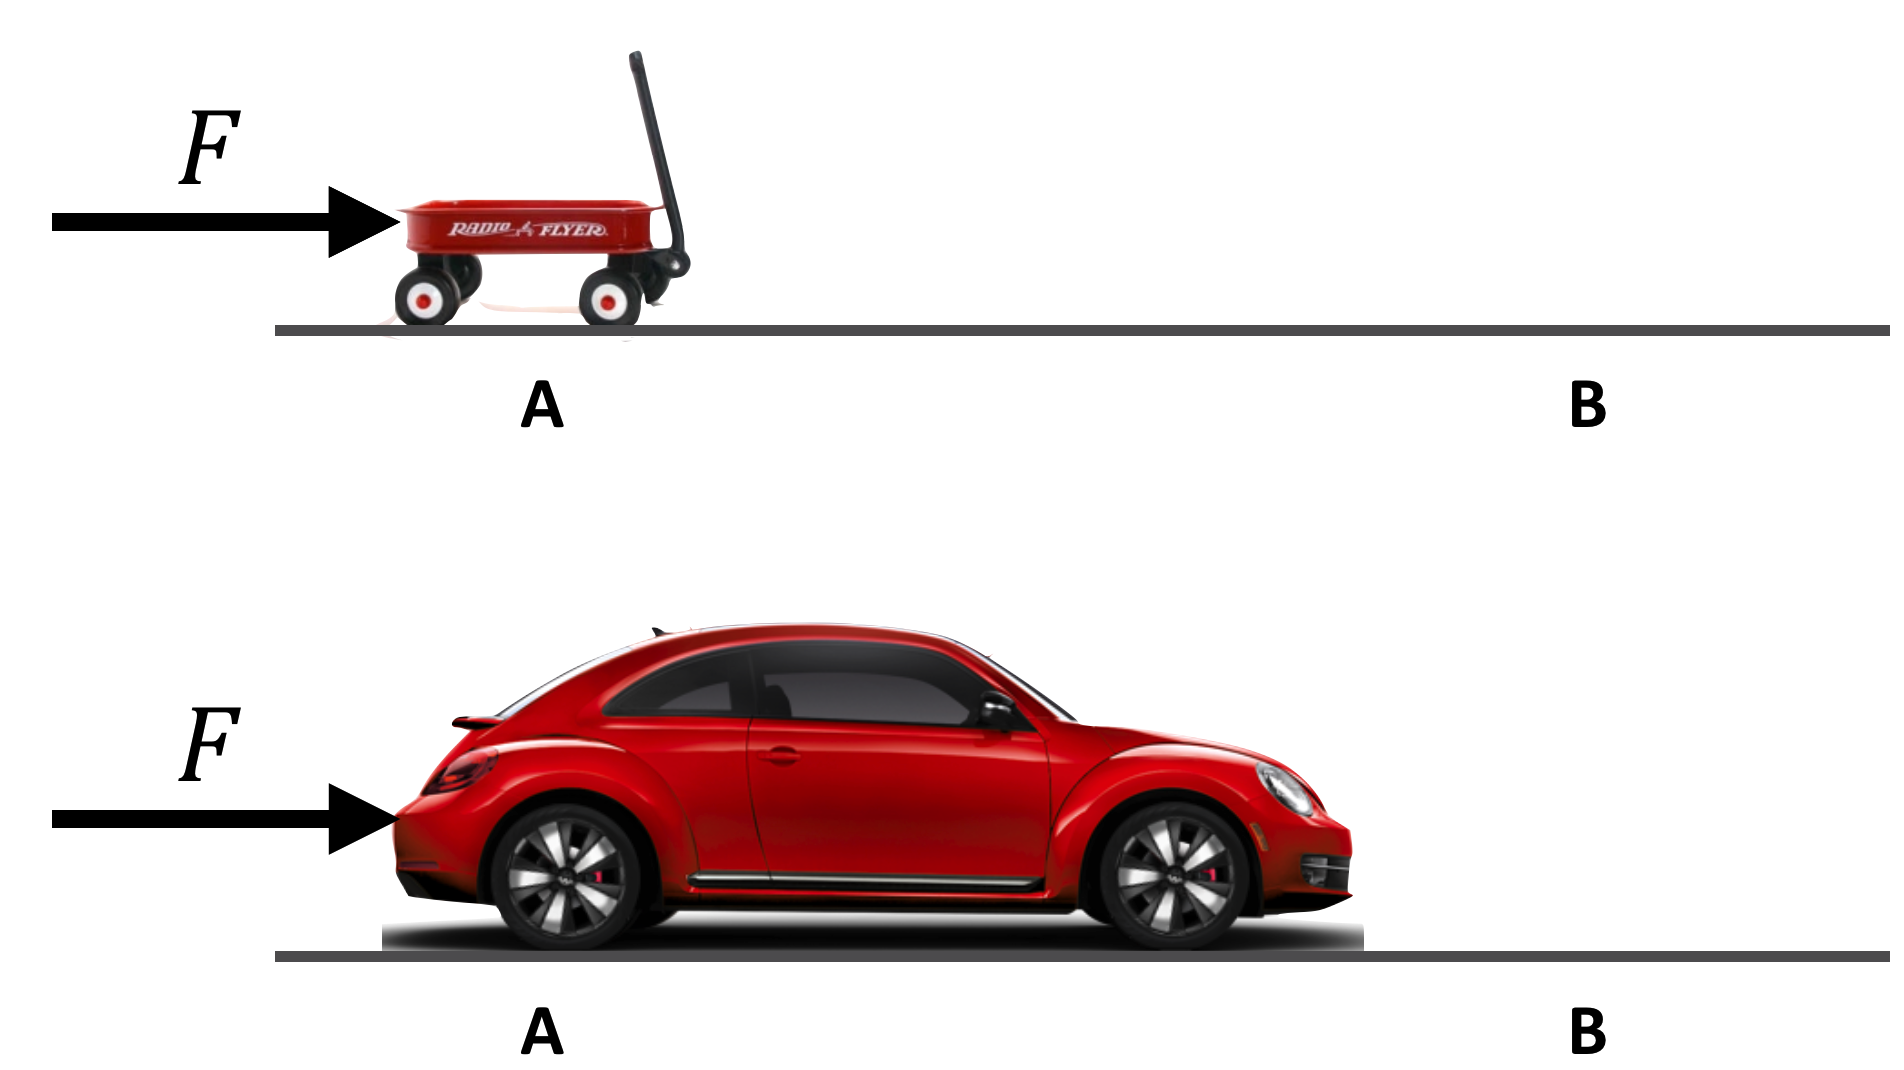
\includegraphics[width=0.8\linewidth,height=\textheight,keepaspectratio]{mechanics/momentum/./iwagon.png}

}

\end{figure}%

}

Will the resulting \(\Delta v\) at point B be the same for both
vehicles?

Of course not. The little red wagon will gain more speed than the
Volkswagen (regardless of its color). The VW is more reluctant to be
accelerated than the wagon. So Equation \eqref{eq:impulse1} is not the
whole story. What's missing is just that reluctance that any object has
to being accelerated, which has a name: \textbf{inertia}.

\section{Newton's Mass}\label{sec-mechmass}

Mass is a toughy and we'll see over and over how complicated it is -- to
the current day. Here's how he defined it in the \emph{Principia}:

``Mass is the quantity of matter arising from its density and bulk
conjointly.''

There you go. Useful? \ldots no?

You do perfectly well to accept the idea that mass is the
\textbf{quantitative measure of an object's reluctance to be coaxed into
changing its motion.}

Here begins our love-hate relationship with mass. This much works:

\begin{tcolorbox}[enhanced jigsaw, toprule=.15mm, opacityback=0, colframe=quarto-callout-important-color-frame, rightrule=.15mm, coltitle=black, bottomtitle=1mm, colbacktitle=quarto-callout-important-color!10!white, bottomrule=.15mm, toptitle=1mm, titlerule=0mm, title={Important}, arc=.35mm, leftrule=.75mm, left=2mm, colback=white, breakable, opacitybacktitle=0.6]

🫵 \emph{Inertia} is an object's resistance to being accelerated and the
measure of an object's inertia is its \emph{mass}.

\end{tcolorbox}

This is the most profound and at the same time, the most mundane idea
that Newton had!

\begin{tcolorbox}[enhanced jigsaw, toprule=.15mm, opacityback=0, colframe=quarto-callout-tip-color-frame, rightrule=.15mm, coltitle=black, bottomtitle=1mm, colbacktitle=quarto-callout-tip-color!10!white, bottomrule=.15mm, toptitle=1mm, titlerule=0mm, title={Tip}, arc=.35mm, leftrule=.75mm, left=2mm, colback=white, breakable, opacitybacktitle=0.6]

🔐 At the deep level of elementary particles, mass confuses us, perhaps
in a different way from how it confuses engineering freshmen. We think
that mass may actually not be an actual property of object, but rather a
result of an object's interaction with a spooky field that sprang into
existence just after the birth of the Universe. Now, in the 21st
century, we've got a whole new set of neuroses about this subject, as
understanding it occupies almost the entire Particle Physics community.
So, Mass has been a problematic subject since its beginning in Newton's
hands.

\end{tcolorbox}

\section{The ``Quantity of Motion'': Momentum}\label{sec-mechmomentum}

We just developed a sense that our hand-built, car-pushing formula,
Equation \eqref{eq:impulse1} has to depend on speed \emph{and} mass and
so we'll just add it in on the right-hand side to get:

\[
\begin{equation}
F\Delta t = m\Delta v  \label{impulse2}
\end{equation}
\]

Being more explicit, when fleshed out impulse is

\[
\begin{equation}
F\Delta t = m(v - v_0) \label{fullimpulse}
\end{equation}
\]

\begin{quote}
There's more to this story To be totally correct, the right hand side of
this equation can be written as \(\Delta (mv)\) which recognizes that
the mass might change instead of, or in addition to, the velocity
changing. This is how a balloon jumps from your hand when you stop
pinching the nozzle, or how a rocket is propelled by ejecting burned
propellent out the back. In each case, the mass of the moving object
changes and that results in a thrust. But we'll not encounter that in
QS\&BB.
\end{quote}

This quantity on the right, \(mv\) is the definition of momentum. So the
impulse is: \$\$ \begin{align}
F\Delta t &= \Delta (mv) \nonumber \\
F\Delta t &= \Delta p \label{momentumdef} \\

\end{align} \$\$

The athletic use of this is instinctive and learned\ldots but with
muscles and your neurosystem not paper and pencil:

\begin{Shaded}
\begin{Highlighting}[]
\CommentTok{\# \#| out.width: “700px”  }
\CommentTok{\# \#| column: screen}
\CommentTok{\#| echo: false}
\NormalTok{knitr}\SpecialCharTok{::}\FunctionTok{include\_graphics}\NormalTok{(}\StringTok{"screenshot\_3684.png"}\NormalTok{)}
\end{Highlighting}
\end{Shaded}

{
\makeatletter
\def\LT@makecaption#1#2#3{%
  \noalign{\smash{\hbox{\kern\textwidth\rlap{\kern\marginparsep
  \parbox[t]{\marginparwidth}{%
    \footnotesize{%
      \vspace{(1.1\baselineskip)}
    #1{#2: }\ignorespaces #3}}}}}}%
    }
\makeatother

\begin{figure}[H]

\sidecaption{\label{fig-impulse_balls}The left-hand version where you
want to change the velocity of a ball for example, in baseball, tennis,
soccer, and golf\ldots anything with a ball. The right-hand version
where you have a fixed goal -- like stopping precisely -- fits football,
gymnastics, and track and field.}

\centering{

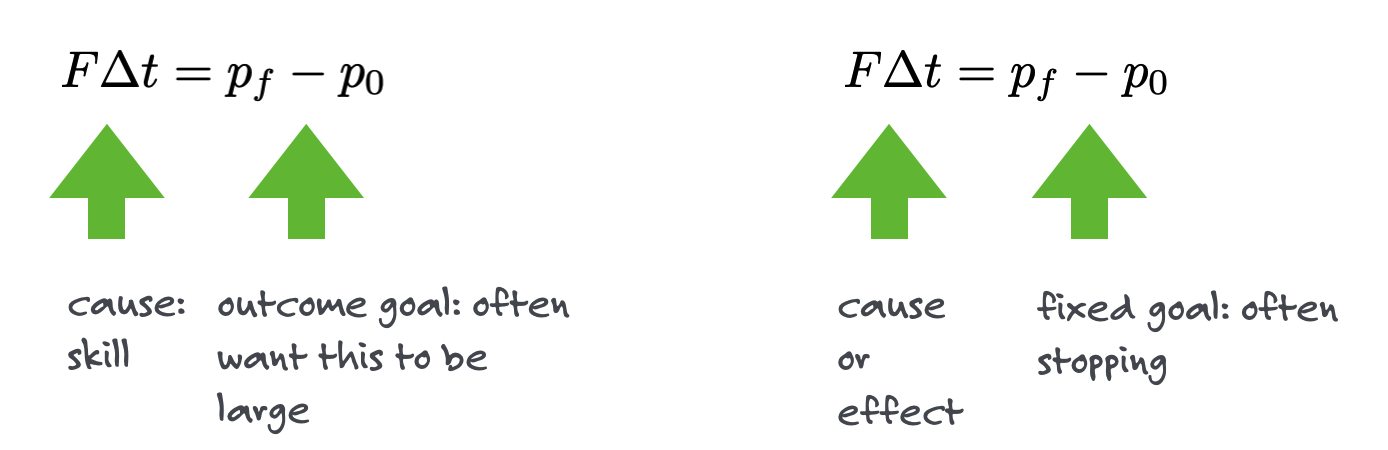
\includegraphics[width=1\linewidth,height=\textheight,keepaspectratio]{mechanics/momentum/screenshot_3684.png}

}

\end{figure}%

}

\begin{center}\rule{0.5\linewidth}{0.5pt}\end{center}

So, repeat after me:

\begin{itemize}
\item
  If there is no net force on an object

  \begin{itemize}
  \item
    it's motion doesn't change

    👉 if its speed was zero\ldots it stays zero

    👉 if its speed was 55 mph\ldots it stays at 55 mph
  \end{itemize}
\end{itemize}

Said another way, if you see the motion of any object changing\ldots{}
then somewhere there is a force actiing (it might be invisible, like a
magnetic field).

One quick change of Equation \eqref{momentumdef}:

\[
\begin{align}
F\Delta t &= \Delta p \nonumber \\
F &= \frac{\Delta p}{\Delta t} \label{newtons2} \\
\text{since }&=\Delta p = \Delta (mv) \nonumber \\
\text{and if the mass is constant } &= \Delta p =m\Delta v \nonumber\\
F &= m \frac{\Delta v}{\Delta t} \nonumber \\
\text{and since } &= \frac{\Delta v}{\Delta t} = a \nonumber \\
F &= ma \label{newtons2b}
\end{align}
\] A couple of these are suitable for a T-shirt: Equation
\eqref{newtons2} is ``Newton's Second law of Motion'' in its most
general physics-major form. Equation \eqref{newtons2b} is the T-shirt
version for motion in which the mass of an object undergoing a push
doesn't change.

\subsection{Newton's 3 laws of motion}\label{sec-newtonslaws}

If there's a second law, there must be a first one and there
is\ldots and a third one. Here they are for completeness:

\begin{enumerate}
\def\labelenumi{\arabic{enumi}.}
\tightlist
\item
  An object with constant velociy will retain that constant velocity of
  zero or another value.
\item
  Best expressed as an equation as \eqref{newtons2}.
\item
  For every force that object A applies to object B, an equal and
  opposite force will be appled by B to A.
\end{enumerate}

The Third law is very useful for solving problems, but that's not what
we're about in \textbf{QS\&BB}.

\subsection{Weight}\label{sec-weight}

There's an important special case of Equation \eqref{newtons2b} which
has to do with the earth and, well, everything that's not nailed down.
The earth attracts all objects with a force (which we'll talk about in a
bit) that seems constant and has a partcular value of acceleration, that
of gravity., We affectionately call it \(g\). So your weight is the
force that the earth applies to you and so we simply have: \[
\begin{align}
F &= ma \text{ ...now modify for gravitational force}\nonumber \\
F &= W \text{ for the special force called "weight"} \nonumber \\
a &= g \text{ for the special acceleration of gravity} \nonumber\\
W &=mg \text{ which is weight on earth} \label{weight}
\end{align}
\] Two caveats:

\begin{enumerate}
\def\labelenumi{\arabic{enumi}.}
\tightlist
\item
  We call this \(g\) ``little g'' and it's only got a specific value for
  the earth. There are different little g's for other planets, moons, or
  stars.
\item
  The force of gravity is actually not constant -- stay tuned. But miles
  above tthe earth it's still so close to \(g\) that we often pretend
  that it's constant.
\end{enumerate}

So little g is an important number:

\begin{itemize}
\tightlist
\item
  In the american system, \(g = 32\) feet/second\(^2\) , 32 ft/s\(^2\)
\item
  For the rest of the world, \(g = 9.8\) meters/second\(^2\), 9.8
  m/s\$\textsuperscript{2}
\end{itemize}

\section{Circular Motion}\label{sec-circular}

Remember that if a velocity changes, then there's an force acting as a
cause and an acceleration is the result. Well, what about driving around
a curve keeping your accelerator at 50 mph? This is the one time in
\textbf{QS\&BB} we'll care about the vector nature of velocity. A true
(for a professional physicist or student) velocity has a magnitude (what
your speedometer reads back) and a direction. So going 50 mph north is a
different velocity than going 50 mph east. Same speed, different
velocity.

Okay, what's going on with you turning that corner where your direction
changes but your speed doesn't. From the formal definition, the velocity
must change 👉 so there must be a force acting 👉 so there is an
acceleration.

It might be easier to think of twirling something overhead. Suppose you
tie a ball to a thin rope and get it rotating above your head in a
horizontal plane, like our little guy in the margin.

\begin{marginfigure}

\centering{

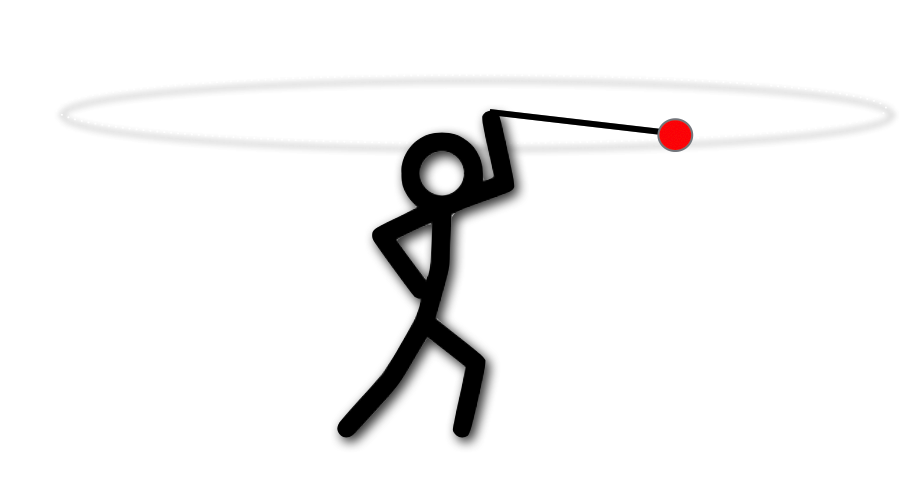
\includegraphics[width=1\linewidth,height=\textheight,keepaspectratio]{mechanics/momentum/screenshot_3696.png}

}

\caption{\label{fig-erad}Twirling a ball over your head in a horizontal
plane.}

\end{marginfigure}%

You can feel a tug. That is, the ball seems to exert a force on your
hand through the rope. But what's really going on is that the ball wants
to go forward (Newton's first law) and you pull it back incrementally,
bit by bit as it goes around. You're supplying that force necessary to
defeat its straight line motion.

This force-towards-the-center is called ``centripetal force'' -- you've
maybe heard of ``centrifugal force'' but that's different and sometimes
called ``ficticious'' which seems sort of insulting. But when you're a
passenger in a car that's going around a curve, you feel a force that's
away from the center of the curve\ldots that's centifugal. But that's
just your body trying to obey that first law and go straight, while
you're in this car going, well, not straight. Where do you get the force
that makes you follow the car? The door against your shoulder, the
friction of the back of your lap on the seat, and hopefully your
seatbelt. Absent those forces which pull you toward the center of the
curve, you'd go flying.

The acceleration that you (or the ball) experience is toward the center
of the circle (which we'll say has radius \(R\), following the direction
of the force, and has its own formula and name of ``centripetal
acceleration'' (\(a_c\)): \[
a_c=\frac{v^2}{R} \label{centripetala}
\] From Newton's second law, there's then a centripetal force. That tug
you provide to the ball of mass \(m\) is: \[
\begin{align}
F_c &= m a_c \nonumber \\
F_c &=m \frac{v^2}{R} \label{centripetalf}
\end{align}
\]

\bookmarksetup{startatroot}

\chapter{Summary}\label{summary}

In summary, this book has no content whatsoever.

\bookmarksetup{startatroot}

\chapter*{References}\label{references}
\addcontentsline{toc}{chapter}{References}

\markboth{References}{References}

\phantomsection\label{refs}
\begin{CSLReferences}{0}{1}
\end{CSLReferences}




\end{document}
